\documentclass[10pt]{article}

%---------------------------------------------------------------------
\usepackage[a4paper, headsep=-4in,bindingoffset=0in,%
left=2.5cm,right=2.5cm,top=2.5cm,bottom=2.5cm,%
footskip=.25in]{geometry}
\newcommand{\textBF}[1]{%
    \pdfliteral direct {2 Tr 0.3 w} %the second factor is the boldness
     #1%
    \pdfliteral direct {0 Tr 0 w}%
}
\usepackage{multirow}
\usepackage{soul}

\usepackage{xr}
\externaldocument{main}
\def\Plus{\texttt{+}}
%\usepackage[english]{babel}   
\usepackage[utf8]{inputenc}  
\usepackage[font=scriptsize]{caption}
\usepackage{tabularx}
%\DeclareCaptionFont{6pt}{\fontsize{6pt}{6pt}\selectfont}
\captionsetup[figure]{font={stretch=1}}  
%\usepackage{sectsty}
\usepackage{subcaption}
\usepackage{wrapfig}
\usepackage{layout}
\usepackage{graphicx}
\usepackage{verbatim}
\usepackage{listings}
\usepackage{mathptmx}

\usepackage{booktabs}
\usepackage{etoolbox}

\newcommand{\beginsupplement}{%
\setcounter{table}{0}
\renewcommand{\thetable}{S\arabic{table}}%
\setcounter{figure}{0}
\renewcommand{\thefigure}{S\arabic{figure}}%
}

\usepackage{lmodern}
\usepackage[T1]{fontenc}
\usepackage[backend=biber,style=apa,sorting=none]{biblatex}
\addbibresource{paperpile.bib}
%\pagenumbering{gobble}
\pagenumbering{arabic}

\graphicspath{{figs/}}
\setlength{\topmargin}{-10pt}
%\renewcommand{\baselinestretch}{1.5}

\usepackage{indentfirst}
\setlength{\parindent}{1cm}
\usepackage[table]{xcolor}
\setlength{\headsep}{1pt}

\begin{document} 

\begin{center}
{\large \section*{Systematic comparison of imaging biomarkers of chronic stroke motor outcome in the ENIGMA Stroke Recovery Working Group dataset}}
\end{center}

\begin{center}
Emily Olafson$^1$, Keith Jamison$^1$, Bethany Lo, Amy Kuceyeski$^1$
\end{center}

    1. \textmd{Department of Radiology, Weill Cornell Medical College, New York City, New York, USA, 10021} 

%---------------------------------------------------------------------

\section{Abstract}
Stroke is a leading cause of physical impairment, and up to a third of stroke survivors have poor motor outcomes five years after the event. However, the ability to predict long-term deficits from acute clinical information remains a challenge. Incorporating information about lesion location can improve prediction models, but it is unclear how to optimally use volumetric lesion data to predict chronic motor outcomes. Several lesion biomarkers have been related to stroke motor outcome, but it is unclear whether they can accurately predict chronic impairments across a range of lesion topographies. Models that incorporate damage to additional sensorimotor regions beyond the primary motor cortex have been shown to explain more variance in post-stroke outcome than models that only incorporate primary motor cortex CST damage. These models typically incorporate damage to premotor, supplementary motor, pre-supplementary motor, and somatosensory cortices. Few studies have assessed the performance of these models with cross-validation. This paper presents a comparison of the predictive accuracy of several imaging biomarkers of post-stroke motor impairment using the ENIGMA dataset, a multi-site stroke lesion database. The models are compared using out-of-sample performance, and the results show that data-driven features outperform theory-driven features. The data-driven features also outperform models trained on chronic subjects when applied to acute subjects. These results highlight the potential of data-driven feature selection in identifying lesion-deficit associations beyond current theory-driven biomarkers.

\section{Introduction}
Stroke is a leading cause of long-term disability worldwide (\cite{Katan2018-qn}), often causing motor impairments that can compromise functional independence. Accurate prognosis in the acute phase of stroke can be used to guide rehabilitation and set treatment goals based on recovery potential, but the ability to predict long-term motor deficits from acute clinical information is still a major challenge.

The location of the lesion in the brain has been related to motor outcomes, but it is unclear how to represent location information in a way that captures the most variance in chronic motor scores. Lesion segmentations, derived from magnetic resonance imaging (MRI) data, reflect the location and size of the lesion in volumetric space, and can be used to determine which neuroanatomical structures were damaged by the stroke. 
Several pre-existing measures of lesion damage can be extracted from binarized lesion segmentations, typically reflecting damage to specific white or gray matter structures, but there is not a consensus on which should be used for predictions of chronic motor deficits. 

Predictive models to date have used input features on the basis of their involvement in motor behavior. The most well-studied biomarker of motor deficits is the corticospinal tract (CST) lesion load, or the proportion of voxels in the ipsilesional corticospinal tract (typically originating from primary motor cortex) that intersect with the lesion (\cite{Zhu2010-qh, Feng2015-du, Findlater2019-je, Lam2018-xh, Pineiro2000-dv}). CST lesion load has been related to motor deficits in the acute and chronic phase of stroke, but CST damage itself is unlikely to capture enough variance in motor deficits in patients with a wide range of lesion topography (for review, see \cite{Kim2017-xe}). Multivariate models that incorporate information about how the lesion damages multiple somatomotor regions like premotor, supplementary, and sensory structures explain more variance in post-stroke motor outcomes than models that only include CST lesion load (\cite{Ito2022-em, Sperber2021-lw, Rondina2016-ds, Rondina2017-ij, Schulz2012-yy}). 

Damage to structures in the somatomotor system have been used as inputs to predictive models because of their causal relationship to motor function; integrity of the CST is necessary for voluntary control of the limbs. However, in context of prediction, where we simply wish to exploit associations between the input data and motor deficits, limiting input features to those in the motor system may curtail predictive accuracy if lesion-deficit associations can also be found outside of those areas. In stroke, structures outside of the motor system may bear predictive value if damage to those structures is consistently associated with motor deficits. Such a phenomenon can occur due to the superposition of the brain's vasculature and spatial maps of motor functions (\cite{Mah2014-cb, Sperber2020-kp,Kasties2021-rm, Calesella2021-kp}). This phenomenon has been well-documented in the field of lesion-deficit inference
(\cite{Mah2014-cb, Sperber2020-kp,Kasties2021-rm, Calesella2021-kp}) and points to the idea that damage to an area (which may itself be outside of the motor system) may be more consistently associated with deficits than damage to an area inside the motor system, and thus may be a more sensitive biomarker of motor deficits. In other words, we may want to  discover useful lesion-deficit associations instead of assuming that pre-established structure-function relationships will have maximal predictive value.

\cite{Bowren2022-rs} discover such associations using lesion-behavior mapping, a technique to identify statistical associations between lesion location anatomy and behavioural deficits. They seed structural connectivity from regions of peak association and use damage to those structural connectivity maps as input to predictive models, in a new cohort. Similarly, \cite{Sperber2021-lw} find that damage to regions identified from lesion-behavior mapping is a more sensitive biomarker of motor deficits than damage to motor areas. This prior work suggests that data-driven feature selection enhances predictive performance. However, using inferential statistics to identify features (i.e. from associative lesion-behavior mapping methods) may fail to identify features that are predictive, i.e., are useful for estimating motor deficits in new subjects (\cite{Bzdok2020-py}).

Machine learning models that select features in a data-driven way in order top optimize out-of-sample performance typically require larger sample sizes that, until recently, been unavailable in stroke research (\cite{Bzdok2020-py}). To our knowledge, only one study to date has used data-driven feature selection to predict post-stroke motor deficits from imaging data \cite{Kasties2021-rm}. Kasties and colleagues perform feature selection with several feature representation strategies (including voxelwise, regional, and lesion-anatomical features) for modelling acute motor impairment to predict acute impairment, albeit with a small sample size (N=100). 

Here, we expand on this work by leveraging the largest stroke imaging database to date containing using a heterogeneous stroke population (N = 789) (\cite{Liew2020-ps}) and directly evaluating different representations of lesion data and feature selection to predict chronic motor deficits. Using the Network Modification tool (\cite{Kuceyeski2013-nk}), we estimated the amount of lesion-induced structural disconnection for each gray matter region in the brain and used data-driven feature selection to identify regions in which structural disconnection was relevant for predicting chronic motor outcomes. Our primary objective was to determine the relative performance of different biomarkers for predicting chronic motor scores, with the hypothesis that data-driven feature selection would improve prediction performance and identify features beyond the current suite of theory-based biomarkers like those in the motor system. As a secondary objective, we assessed whether predictive performance could be improved by incorporating demographic information and by combining predictions from several different biomarkers using ensemble models.

\section{Materials and methods}
\subsection{Sample demographics}
A subset of cross‐sectional data from the Enhancing Neuroimaging Genomics through Meta Analysis (ENIGMA) Stroke Recovery Working Group database (available as of 10 Sept. 2021) was used in the study. Details of the ENIGMA Stroke Recovery procedures and methods are available in (\cite{Liew2020-ps}). The data originated from 22 research studies (sites) (Table \ref{table:Demographics}). Informed consent was obtained from all subjects, and data were collected in compliance with each institution’s local ethical review boards and in accordance with the Declaration of Helsinki.

ENIGMA Stroke Recovery participants with the following data were included: (1) high‐resolution (1‐mm isotropic) T1‐weighted brain MRI (T1w) acquired with a 3T MRI scanner; (2) information about time since stroke at time of imaging (3) age, (4), sex, and (5) assessment of motor function from one of several tests: Fugl Meyer Assessment of Upper Extermities (FMA‐UE) (\cite{Gladstone2002-fw}); the Action Research Arm test (ARAT) which tests arm function through assessment of the timing and difficulty of motor task completion (\cite{Yozbatiran2008-xv}); the Barthel index, which measures the extent to which somebody can function independently and has mobility in their activities of daily living (\cite{Sulter1999-rr}); National Institutes of Health Stroke Score (NIHSS), a broad measure of stroke severity that includes assessment of non-motor and motor functions (\cite{Lyden2017-za}. For a majority of the chronic subjects (76$\%$), motor deficits are normalized FMA‐UE scores, whereas  normalized FMA‐UE scores were available for only $12\%$ of the acute data (for full breakdown of type of test used for each site in the dataset, see Table \ref{motor_scores}). Motor scores were normalized by dividing by the raw score by the maximum possible score on the assessment. Behavioral data were collected within approximately 72 hours of the MRI. Subjects were considered in the chronic phase of stroke if their time since stroke was greater than 180 days, and considered in the acute phase if their time since stroke was less than 180 days (\cite{Bernhardt2017-av}). Subjects with cortical and subcortical lesions were included in the study; lesions were not flipped (see Supplementary Figure \ref{lesiondist} for lesion distribution in MNI space). 

\newpage
\begin{table}[h]
\centering
\caption{Site breakdown of total sample size (N), number of females (F) and males (M), and information about age (years), normed motor scores, time since stroke (days), and lesion volume ($cm^3$). IQR, interquartile range}

\label{table:Demographics}
\begin{tabular}{llllll}
\toprule
Site ID & Total N. & Median age (y) & Median motor  & Median time    & Median lesion vol. \\
& (F/M) & (IQR) & score (IQR) &  since stroke  & ($cm^3$) (IQR) \\
 \textbf{Acute}  & & & & (mos.) (IQR) & \\
\arrayrulecolor{black!30}\midrule
r005 & 1 (0/1) & 50.0 (0.0) & 0.29 (0.00) & 5.1 (0.0) & 1.69 (0.00) \\
r009 & 50 (13/37) & 70.0 (18.5) & 1.00 (0.05) & 0.2 (0.1) & 1.65 (6.96) \\
r025 & 9 (4/5) & 70.0 (19.0) & 1.00 (0.09) & 3.0 (1.0) & 0.52 (1.44) \\
r028 & 1 (0/1) & 63.0 (0.0) & 0.74 (0.00) & 5.5 (0.0) & 23.87 (0.00) \\
r031 & 36 (10/26) & 58.5 (13.2) & 0.52 (0.38) & 4.5 (1.7) & 10.83 (38.77) \\
r038 & 72 (30/42) & 66.5 (21.2) & 0.78 (0.66) & 2.9 (2.3) & 11.53 (41.64) \\
r040 & 57 (32/25) & 64.0 (22.0) & 0.40 (0.50) & 1.8 (1.5) & 14.72 (58.63) \\
r047 & 2 (1/1) & 71.0 (2.0) & 0.59 (0.26) & 4.4 (0.2) & 23.78 (19.19) \\
r049 & 21 (12/9) & 65.0 (16.0) & 0.95 (0.00) & 0.0 (0.0) & 1.30 (2.18) \\
r050 & 14 (7/7) & 68.0 (16.8) & 0.92 (0.10) & 0.0 (0.0) & 0.33 (0.40) \\
r053 & 52 (20/32) & 63.5 (20.5) & 0.92 (0.17) & 3.0 (3.0) & 13.50 (28.27) \\
r054 & 12 (5/7) & 65.5 (11.8) & 0.67 (0.83) & 0.4 (0.2) & 4.06 (14.15) \\
 & & & & &\\
\textbf{Chronic}  & & & & &\\
\arrayrulecolor{black!30}\midrule
r001 & 39 (10/29) & 61.0 (17.0) & 0.65 (0.23) & 23.5 (40.0) & 6.27 (18.06) \\
r002 & 12 (6/6) & 69.5 (11.5) & 0.50 (0.41) & 73.2 (51.9) & 28.24 (31.71) \\
r003 & 15 (6/9) & 61.0 (16.5) & 0.24 (0.20) & 48.8 (67.6) & 20.28 (76.88) \\
r004 & 19 (7/12) & 44.0 (14.5) & 0.17 (0.16) & 50.4 (81.9) & 36.85 (44.29) \\
r005 & 27 (12/15) & 66.0 (16.5) & 0.79 (0.45) & 31.4 (27.8) & 1.61 (40.27) \\
r009 & 60 (17/43) & 71.0 (7.2) & 0.96 (0.12) & 27.4 (9.3) & 1.43 (4.65) \\
r025 & 16 (3/13) & 64.5 (13.2) & 0.98 (0.58) & 14.2 (10.2) & 5.92 (14.26) \\
r027 & 28 (8/20) & 57.0 (10.2) & 0.30 (0.16) & 19.3 (24.7) & 12.30 (62.13) \\
r028 & 21 (6/15) & 63.0 (9.0) & 0.82 (0.24) & 26.5 (37.5) & 5.25 (41.28) \\
r031 & 1 (0/1) & 52.0 (0.0) & 0.68 (0.00) & 6.1 (0.0) & 1.54 (0.00) \\
r034 & 15 (6/9) & 58.4 (11.1) & 0.82 (0.20) & 61.3 (68.3) & 6.68 (34.99) \\
r035 & 15 (6/9) & 64.0 (18.0) & 0.64 (0.52) & 33.5 (22.9) & 3.89 (31.56) \\
r038 & 18 (7/11) & 67.0 (10.0) & 1.00 (0.12) & 15.1 (10.1) & 1.98 (1.63) \\
r040 & 14 (7/7) & 63.5 (9.8) & 0.68 (0.47) & 14.1 (17.5) & 8.65 (82.65) \\
r042 & 22 (11/11) & 48.5 (15.5) & 0.64 (0.19) & 29.6 (36.4) & 14.16 (49.53) \\
r044 & 4 (0/4) & 68.0 (9.2) & 0.52 (0.25) & 43.7 (52.9) & 23.65 (67.00) \\
r045 & 4 (1/3) & 62.0 (5.2) & 0.49 (0.24) & 96.1 (59.0) & 7.97 (6.66) \\
r046 & 11 (3/8) & 62.0 (10.5) & 0.50 (0.29) & 86.3 (83.4) & 4.62 (19.82) \\
r047 & 44 (14/30) & 65.5 (12.0) & 0.65 (0.44) & 38.1 (53.7) & 12.72 (41.33) \\
r048 & 43 (16/27) & 68.0 (12.5) & 0.79 (0.44) & 46.2 (49.8) & 7.93 (43.45) \\
r052 & 32 (12/20) & 63.0 (13.5) & 0.41 (0.09) & 39.1 (42.2) & 6.98 (51.55) \\
 & & & & &\\
\textbf{All}  & & & & &\\
\arrayrulecolor{black!30}\midrule
& 789 (293/496) & 64.0 (18.0) & 0.7 (0.5) & 12.2 (0.2) & 6.45 (32.48) \\
\bottomrule
\end{tabular}
\end{table}

\subsection{General overview}

We built several models to predict chronic motor scores from imaging data and minimal clinical information. Each model uses lesion-derived information to predict normalized motor scores. We compared several different structural damage measures, including lesion load, reflecting damage to the sensorimotor system, and measures of structural disconnection reflecting damage to gray matter regions across the entire brain. Nested cross-validation was performed for all measures to train models and assess performance on unseen data. We assessed whether feature selection improved performance for models using whole-brain measures of structural disconnection. Notably, we evaluated whether including acute subjects in the training set (but not in the test set) improved prediction of chronic deficits, with the idea that the signal in the acute data would be useful in predicting deficits in the chronic phase. We also evaluated whether basic clinical information (age, sex, time since stroke) improved performance on top of lesion information using ensemble models. Finally, we assessed whether ensemble models averaging predictions from all models improved performance. 

\subsubsection*{Machine learning framework}
Regression models were trained and evaluated using repeated 5-fold nested cross-validation loop. Models differed for each lesion biomarker based on the data; see below for implementation details for each biomarker. In the outer loop, the data was split into 5 training and test partitions. Using only chronic data to train the models, there were approximately 370 subjects in the training set and 92 subjects in the test set. If acute data was used in training, it was added to the training partition, such that there were 696 subjects in the training set and 92 subjects in the test set. Training data was further partitioned into training and validation sets in the inner loop, and if hyperparameters were specified in the model, they were optimized in the inner loop. 

Out-of-sample performance was calculated as the average performance across 5 outer test folds. We obtained a distribution of out-of-sample performance by splitting the data into 5 train/test folds 100 times, shuffling the indices of the splits each time. 

\subsubsection*{Model performance}
Model performance was assessed by comparing true normalized motor scores with predicted scores. Performance was calculated with Pearson's correlation coefficient and by the explained variance score, or $R^2$, which captures the percent of variation in motor scores explained by variation in the model predictors. Two performance metrics were used in order to compare results with prior literature, which uses both.

\subsection{Description of models and their inputs}
\subsubsection*{Primary motor cortex CST lesion load (M1-CST-LL) models}

The lesion load of the corticospinal tract originating from the primary motor cortex (M1-CST-LL) has been associated with motor impairment in several stroke studies. Here, as in previous work, M1-CST-LL was calculated as the proportion of lesioned voxels intersecting with a binarized ipsilesional M1-CST template (\cite{Zhu2010-qh}). Specifically, lesion load was calculated in 1mm MNIv6 space as:
\begin{equation}
    \textit{Lesion load} = \frac{\textit{Number of lesioned voxels intersecting with  tract}}{\textit{Number of voxels in tract}}
\end{equation}
Left and right hemisphere M1-CST segmentations in MNI space were obtained from the high-resolution sensorimotor area tract template (SMATT) (\cite{Archer2018-ti}). In this dataset, M1-CST Lesion load had a heavy-taiedl distribution (Supplementary Figure \ref{lesion_load_dist}a).
Linear regression was used to model the relationship between ipsilesional M1-CST-LL and chronic motor scores. The weights from best-performing model in the inner loop were used to predict motor scores for new subjects in the test folds. 

\subsubsection*{Sensorimotor tract lesion load  (SMATT-LL) models}
Sensorimotor tract segmentations were obtained from the sensorimotor area tract template (SMATT) (\cite{Archer2018-ti}), a set of 12 tracts derived from probabilistic tractography seeded in the left and right primary motor cortex (M1), dorsal and ventral premotor cortex (PMd and PMv, respectively), supplementary motor area (SMA), pre-supplementary motor area (pre-SMA), and primary somatosensory cortex (S1) of healthy controls (Figure \ref{smatt}). Lesion load was calculated as above, for all 12 tracts (i.e. separately for left and right hemispheres) and for 6 ipsilesional tracts. Left and right SMATT lesion load was calculated in order to assess whether preserving hemispheric information improved predictions. For subjects with brainstem, cerebellar, and/or bilateral cerebral strokes, ipsilesional lesion load was calculated as the average lesion load of the left and right hemisphere tracts. Lesion loads also had a heavy-tailed distribution (Supplementary Figure \ref{lesion_load_dist}b,c). 

\begin{figure}[ht]
    \centering
    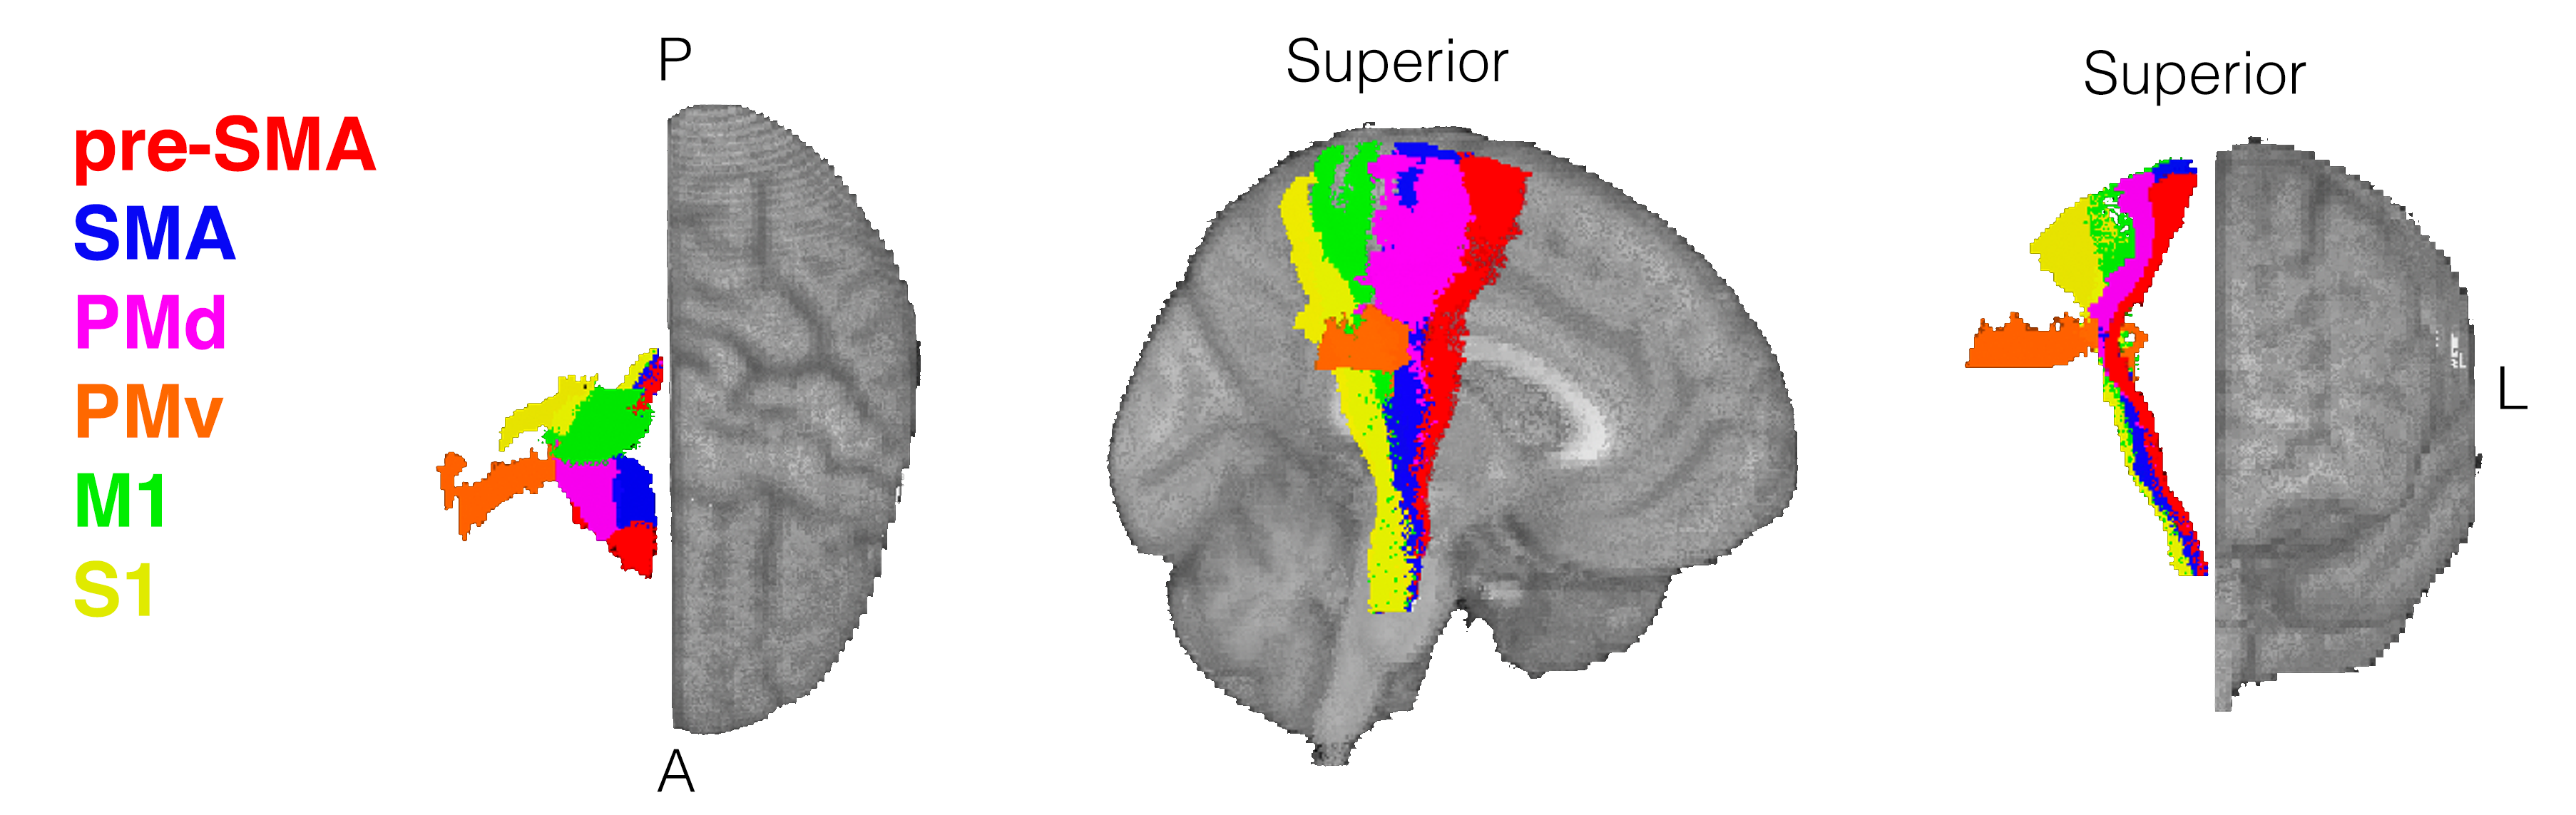
\includegraphics[width=0.7\linewidth]{figures/SMATT.png}
    \caption{Sensorimotor tract template atlas (SMATT), displaying only right hemisphere tracts. Includes supplementary motor area (SMA), dorsal premotor cortex (PMd), ventral premotor cortex (PMv), pre-supplementary motor area (pre-SMA), primary sensory cortex (S1),  and primary motor cortex (M1).}
    \label{smatt}
\end{figure}


Ridge regression models were used to predict chronic motor deficits from ipsilesional SMATT lesion loads (6 features) and from left/right hemisphere SMATT lesion loads (12 features). Ridge regression was used to account for multicollinearity of lesion load values between tracts (Supplementary Figure \ref{smatt_pairwise_correlations}, \ref{smatt_pairwise_correlations_bi}). Lesion load values were normalized (after train/test split) by subtracting the mean across subjects and dividing by the l2-norm prior to model fitting. In the inner loop, the degree of regularization on regression coefficients ($\lambda$) was determined via. grid-search, searching over 30 values ranging [$10^-2$ to $10^2$]. The training data was fit with the selected $\lambda$ and this model was used to predict motor scores for new subjects in the test folds.


\subsubsection*{Regional change in connectivity (ChaCo) models}
Lesion masks in $1mm^3$ MNI v6 space were processed with the Network Modification Tool (NeMo Tool) v2 pipeline (\cite{Kuceyeski2013-nk}) (https://github.com/kjamison/nemo for more detailed information). Given a lesion mask, the NeMo tool produces outputs that reflect the impact of the lesion on the white matter tracts connecting brain regions. The NeMo tool identifies every white matter streamline that intersects with a lesion and determines the brain regions at the endpoints of those streamlines, whose structural connections are putatively disrupted (Figure \ref{nemo}). The NeMo tool uses a reference structural connectome dataset of 420 unrelated subjects from the Human Connectome Project (HCP) Young Adult database. Structural connectivity for HCP subjects was obtained using deterministic tractography (SD stream) with dynamic seeding, with additional SIFT2 weighting for each of 5 million streamlines (\cite{Smith2015-eb}). Regional change in connectivity (ChaCo) scores, or the ratio of the number of disrupted streamlines divided by the total number of streamlines for each region, were calculated for all grey matter regions (see Figure \ref{sumchaco_acutechronic} for distribution of ChaCo scores across subjects). Regional ChaCo scores from two different altases were compared: the 86-region Desikan-Killiany Atlas (68 cortical regions $\Plus$ 18 subcortical regions, excluding brainstem) from FreeSurfer ("fs86" for short), which contains coarse anatomically parcellated regions (\cite{Desikan2006-vf,Fischl2002-lb}), and the 268-region Shen atlas ("shen268" for short), which contains more fine-grained functionally parcellated cortical and subcortical regions (\cite{Shen2013-zn}).

\begin{figure}[ht]
  \centering
  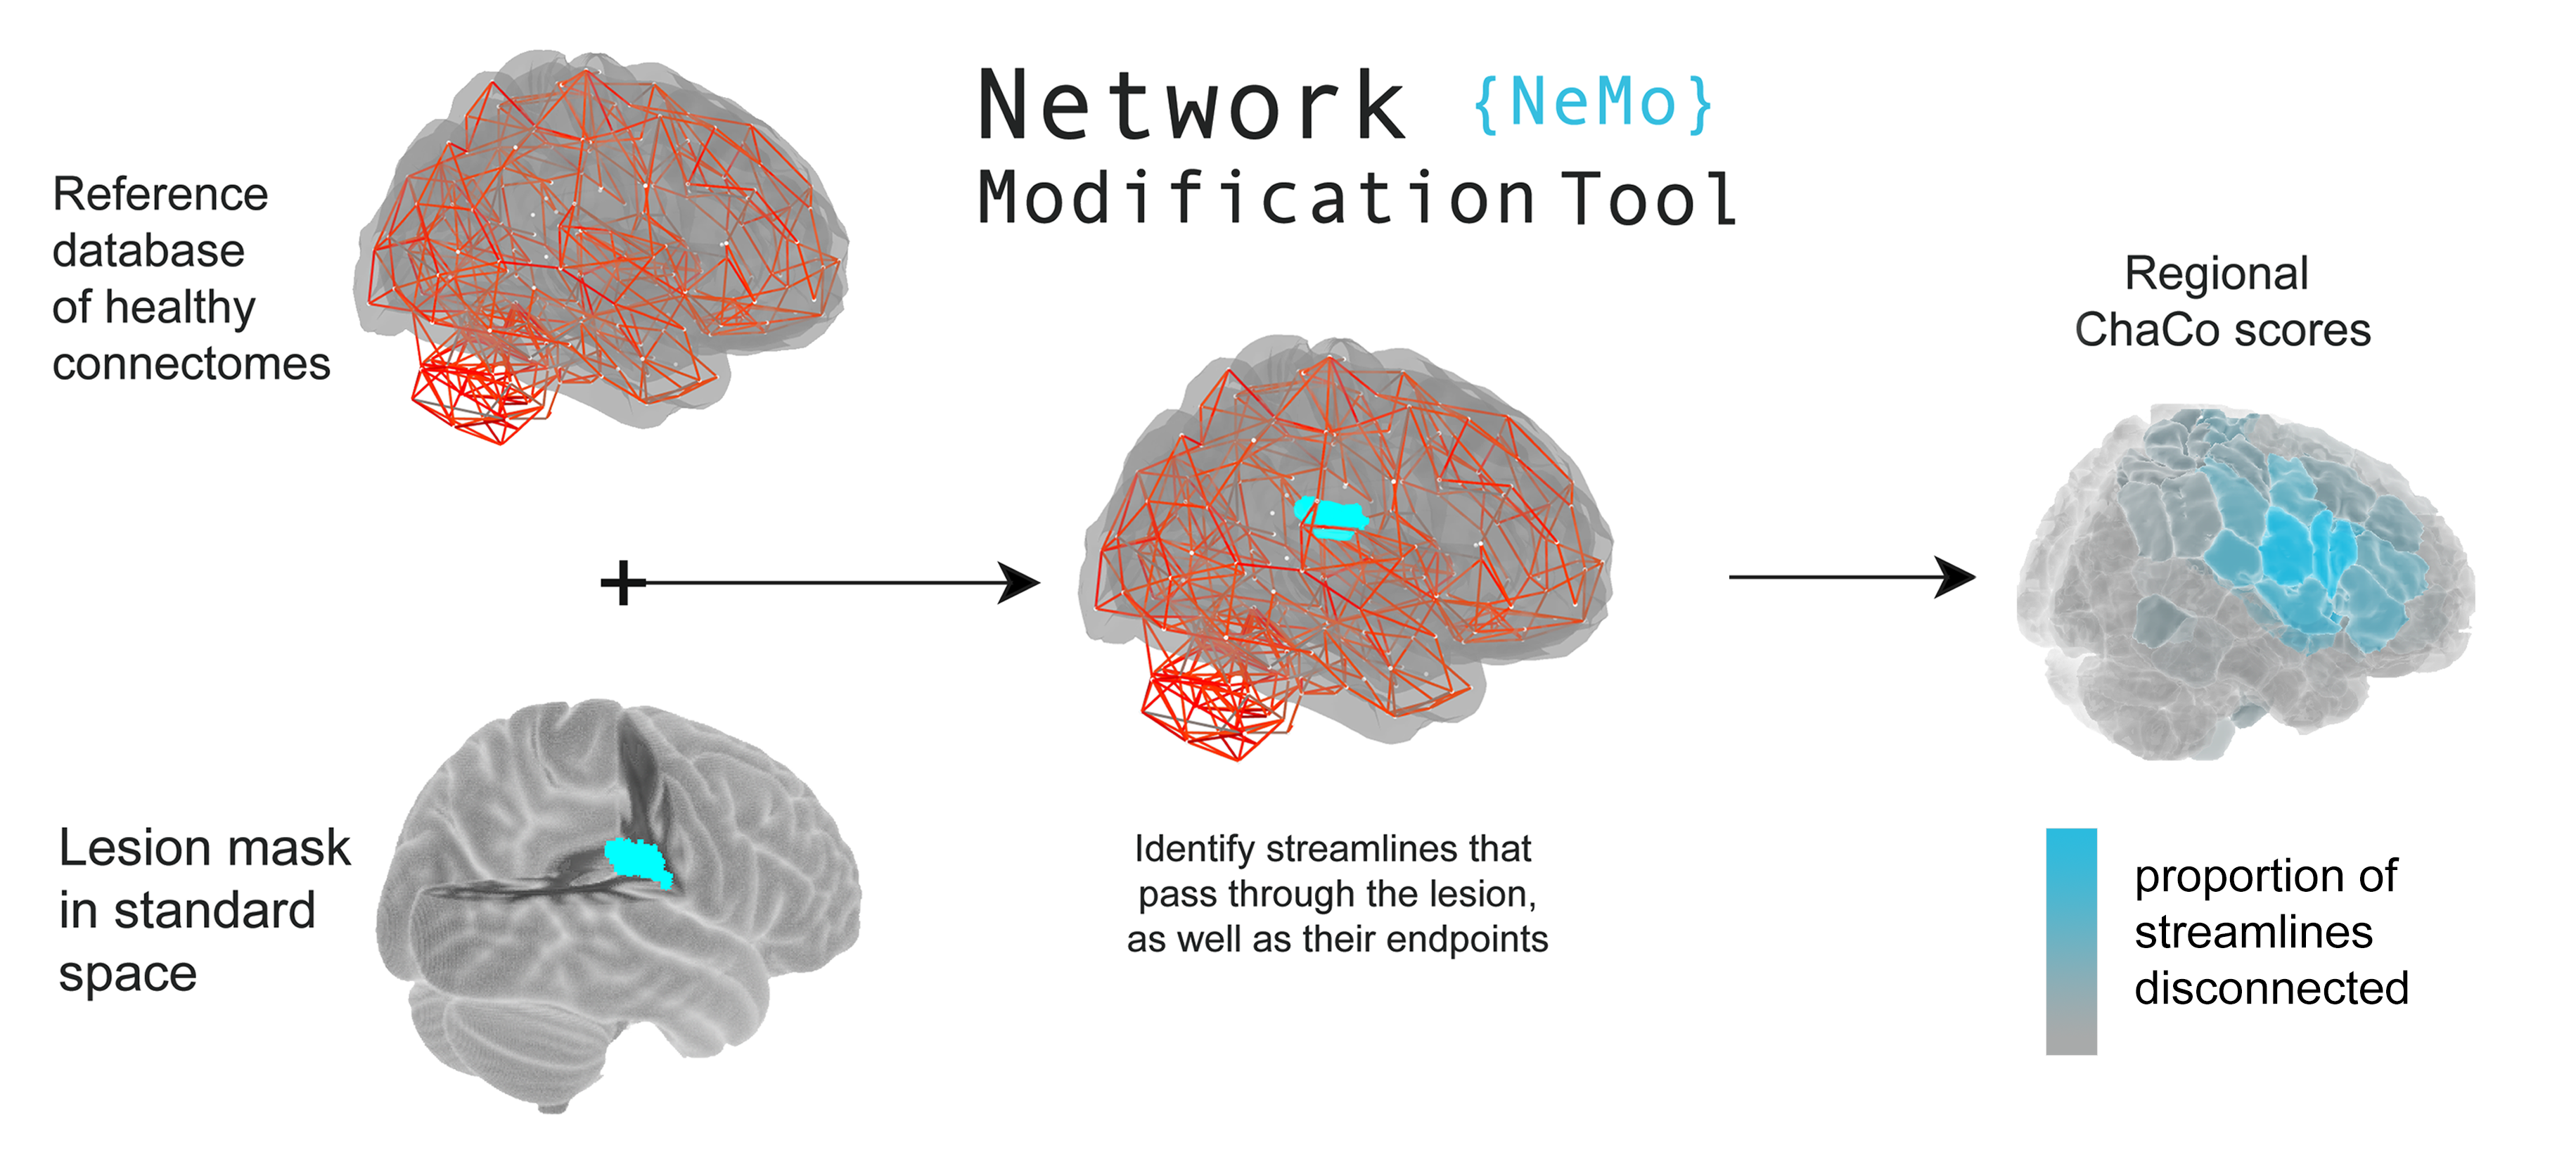
\includegraphics[width=1\linewidth]{figures/Multi-panelML_white_regional.png}
  \caption{Overview of the Network Modification tool. Binary lesion masks in MNI space representing the presence of a stroke lesion (turquoise) in a given voxel are provided by the user. Each lesion mask is embedded into 420 unrelated healthy structural connectomes (separately for each healthy subject) and the regional or pairwise change in connectivity (ChaCo) scores are calculated and averaged across healthy subjects (parcellation shown here is the Shen 268-region atlas). }
  \label{nemo}
\end{figure}

Two flavors of models using ChaCo scores were assessed to determine the benefits of performing feature selection. First, ridge regression models were assessed, as described above, with whole-brain regional ChaCo scores as inputs (86 features for the fs86 atlas, 268 features for the shen268 atlas). Second, a filter-based feature selection step was added to ridge regression models to obtain a subset of features that were the most useful for prediction (\cite{Hall1999-qr, Pudjihartono2022-zg}). We mixed hyperparameter tuning and feature selection in the same step, considering the number of features as a hyperparameter itself. Features were ranked by their their association with the outcome variable (p-value from univariate correlation). In the inner loop, both the amount of regularization on regression coefficients ($\lambda$) and the number of features to retain in the feature selection step ($\kappa$) were selected via. grid search. The $\lambda$ value was chosen by searching over 30 values ranging [$10^-2$ to $10^2$], and the $\kappa$ value was chosen by searching 30 values ranging from 5 to the maximum number of features possible (for fs86: 86, for shen268: 268) in base-2 steps. 

\subsubsection*{Ensemble models}

We tested whether models including demographic information (age, sex, and days post stroke) alongside lesion data will perform better than models with lesion data or demographic data alone (i.e., variance explained from lesion data and demographic data is not redundant). We also assessed whether models including both lesion load and ChaCo scores will perform better than models with lesion load or ChaCo scores alone. We used ensemble models that average predictions from different learners (\cite{Hastie2001-or}); the idea of ensemble learning is to build a single prediction model by combining the strengths of a collection of simpler base models. 

Ensemble models were generated by training ChaCo-models and lesion load models separately, on the same subjects and with the same training/test/validation splits, and averaging the final predicted scores for each subject. A standard linear regression model was used to model the relationship between demographic information and motor impairment. 

\subsubsection*{Code availability}
All analysis scripts that generated the results of the present study are readily accessible and open for reuse (https://github.com/emilyolafson/lesion$\_$predictions). The script can be easily modified to predict any outcome score from ChaCo scores/lesion load data.

\section{Results}
The relative out-of-sample performances of the models can be found in Figure \ref{analysis1}.

The models that best predicted chronic motor scores in unseen subjects were a ridge regression model with correlation-based feature selection using regional ChaCo scores from the shen268-region atlas, using acute and chronic data for training (correlation = 0.467, $R^2$ = 0.210), and a ridge regression model without feature selection using regional ChaCo scores from the 86-region FreeSurfer atlas, using acute and chronic data for training (correlation = 0.458, $R^2$ = 0.204, n.d. between models). Models M1 CST-LL, SMATT-LL, and sLNM-LL performed worse on average than ChaCo models, with SMATT-LL models using only chronic data for training performing the best among them (correlation = 0.446, $R^2$ = 0.188) and M1 CST-LL models performing the worst (correlation = 0.395, $R^2$ = 0.133, n.d. between chronic and mixed training data). 

Features selected in at least 250/500 outer folds of the ChaCo models are shown in (Figure \ref{analysis1}D and \ref{analysis1_posweights} for negative and positive weights, respectively).

On average, around 110 features were chosen for the shen268 ChaCo models (Figure \ref{lambda_kappa}). A hierarchically-clustered heatmap of the correlation matrix of the selected features (Figure \ref{heatmap_shen}) suggests that while many of the selected features are clustered and possibly redundant (i.e., there is high inter-feature correlation across subjects), there are several standalone regions that are consistently incorporated into the model. 

\newpage 
\newpage

\begin{table}[h]
\centering
\label{table:5}
\begin{tabular}{lrrll}
\toprule
 &  & \multicolumn{2}{c}{Median performance} \\
Ensemble type & Model name & Correlation & $R^2$  \\
\midrule
\multirow[t]{8}{*}{None (Lesion load or} & M1 CST-LL & 0.395 & 0.133 \\
 ChaCo only)& Ipsi. CST-LL & 0.430 & 0.174 \\
 & L/R CST-LL & 0.446 & 0.188 \\
 & sLNM-LL & 0.427 & 0.165 \\
 & ChaCo (fs86) & 0.458 & 0.204 \\
 & ChaCo (shen268) & 0.456 & 0.199 \\
 & ChaCo (fs86) (feat. select.) & 0.447 & 0.191 \\
 & ChaCo (shen268) (feat. select.) & 0.467 & 0.210 \\
\multirow[t]{16}{*}{Lesion load $\Plus$} & M1 CST-LL + ChaCo (fs86subj) & 0.461 & 0.210 \\
 ChaCo & M1 CST-LL + ChaCo (shen268) & 0.463 & 0.211 \\
 & Ipsi. CST-LL + ChaCo (fs86subj) & 0.478 & 0.226 \\
 & Ipsi. CST-LL + ChaCo (shen268) & 0.481 & 0.228 \\
 & L/R CST-LL + ChaCo (fs86subj) & 0.481 & 0.227 \\
 & L/R CST-LL + ChaCo (shen268) & 0.481 & 0.228 \\
 & sLNM-LL + ChaCo (fs86subj) & 0.468 & 0.214 \\
 & sLNM-LL + ChaCo (shen268) & 0.472 & 0.217 \\
 & M1 CST-LL + ChaCo (fs86subj) (feat. select.) & 0.458 & 0.206 \\
 & M1 CST-LL + ChaCo (shen268) (feat. select.) & 0.469 & 0.217 \\
 & Ipsi. CST-LL + ChaCo (fs86subj) (feat. select.) & 0.476 & 0.223 \\
 & Ipsi. CST-LL + ChaCo (shen268) (feat. select.) & 0.485 & 0.233 \\
 & L/R CST-LL + ChaCo (fs86subj) (feat. select.) & 0.475 & 0.222 \\
 & L/R CST-LL + ChaCo (shen268) (feat. select.) & 0.486 & 0.232 \\
 & sLNM-LL + ChaCo (fs86subj) (feat. select.) & 0.462 & 0.208 \\
 & sLNM-LL + ChaCo (shen268) (feat. select.) & 0.474 & 0.222 \\
\multirow[t]{8}{*}{Demographics} & M1 CST-LL + demog. & 0.424 & 0.173 \\
 & Ipsi. CST-LL + demog. & 0.457 & 0.199 \\
 & L/R CST-LL + demog. & 0.462 & 0.203 \\
 & sLNM-LL + demog. & 0.452 & 0.191 \\
 & ChaCo (fs86) + demog & 0.471 & 0.203 \\
 & ChaCo (shen268) + demog & 0.468 & 0.204 \\
 & ChaCo (fs86) (feat. select.) + demog & 0.465 & 0.201 \\
 & ChaCo (shen268) (feat. select.) + demog & 0.481 & 0.215 \\
\multirow[t]{16}{*}{Lesion load $\Plus$} & M1 CST-LL + ChaCo (fs86subj) + demog. & 0.476 & 0.214 \\
 ChaCo $\Plus$ & M1 CST-LL + ChaCo (shen268) + demog. & 0.477 & 0.216 \\
 Demographics & Ipsi. CST-LL + ChaCo (fs86subj) + demog. & 0.492 & 0.230 \\
 & Ipsi. CST-LL + ChaCo (shen268) + demog. & 0.495 & 0.232 \\
 & L/R CST-LL + ChaCo (fs86subj) + demog. & 0.494 & 0.231 \\
 & L/R CST-LL + ChaCo (shen268) + demog. & 0.494 & 0.232 \\
 & sLNM-LL + ChaCo (fs86subj) + demog. & 0.484 & 0.222 \\
 & sLNM-LL + ChaCo (shen268) + demog. & 0.487 & 0.224 \\
 & M1 CST-LL + ChaCo (fs86subj) (feat. select.) + demog. & 0.472 & 0.212 \\
 & M1 CST-LL + ChaCo (shen268) (feat. select.) + demog. & 0.482 & 0.222 \\
 & Ipsi. CST-LL + ChaCo (fs86subj) (feat. select.) + demog. & 0.490 & 0.228 \\
 & Ipsi. CST-LL + ChaCo (shen268) (feat. select.) + demog. & 0.498 & 0.237 \\
 & L/R CST-LL + ChaCo (fs86subj) (feat. select.) + demog. & 0.490 & 0.229 \\
 & L/R CST-LL + ChaCo (shen268) (feat. select.) + demog. & 0.499 & 0.237 \\
 & sLNM-LL + ChaCo (fs86subj) (feat. select.) + demog. & 0.479 & 0.218 \\
 & sLNM-LL + ChaCo (shen268) (feat. select.) + demog. & 0.492 & 0.230 \\
 
 \arrayrulecolor{black}\bottomrule
\end{tabular}
\caption{Test performance of all models evaluated, displaying median $R^2$ and median correlation of average hold-out performances (i.e. average across 5 outer folds) across 100 permutations. Demog. = demographics, Ipsi. = Ipsilesional, SMATT LL = sensorimotor tract template lesion load, L/R SMATT LL = left and right sensorimotor tract template lesion load, M1 CST LL = M1 corticospinal tract lesion load, ChaCo = Change in Connectivity, fs86 = FreeSurfer 86-region atlas, feat. select. = feature selection}
\label{results_table_acutechronic}

\end{table}



\begin{figure}[htp]
\centering
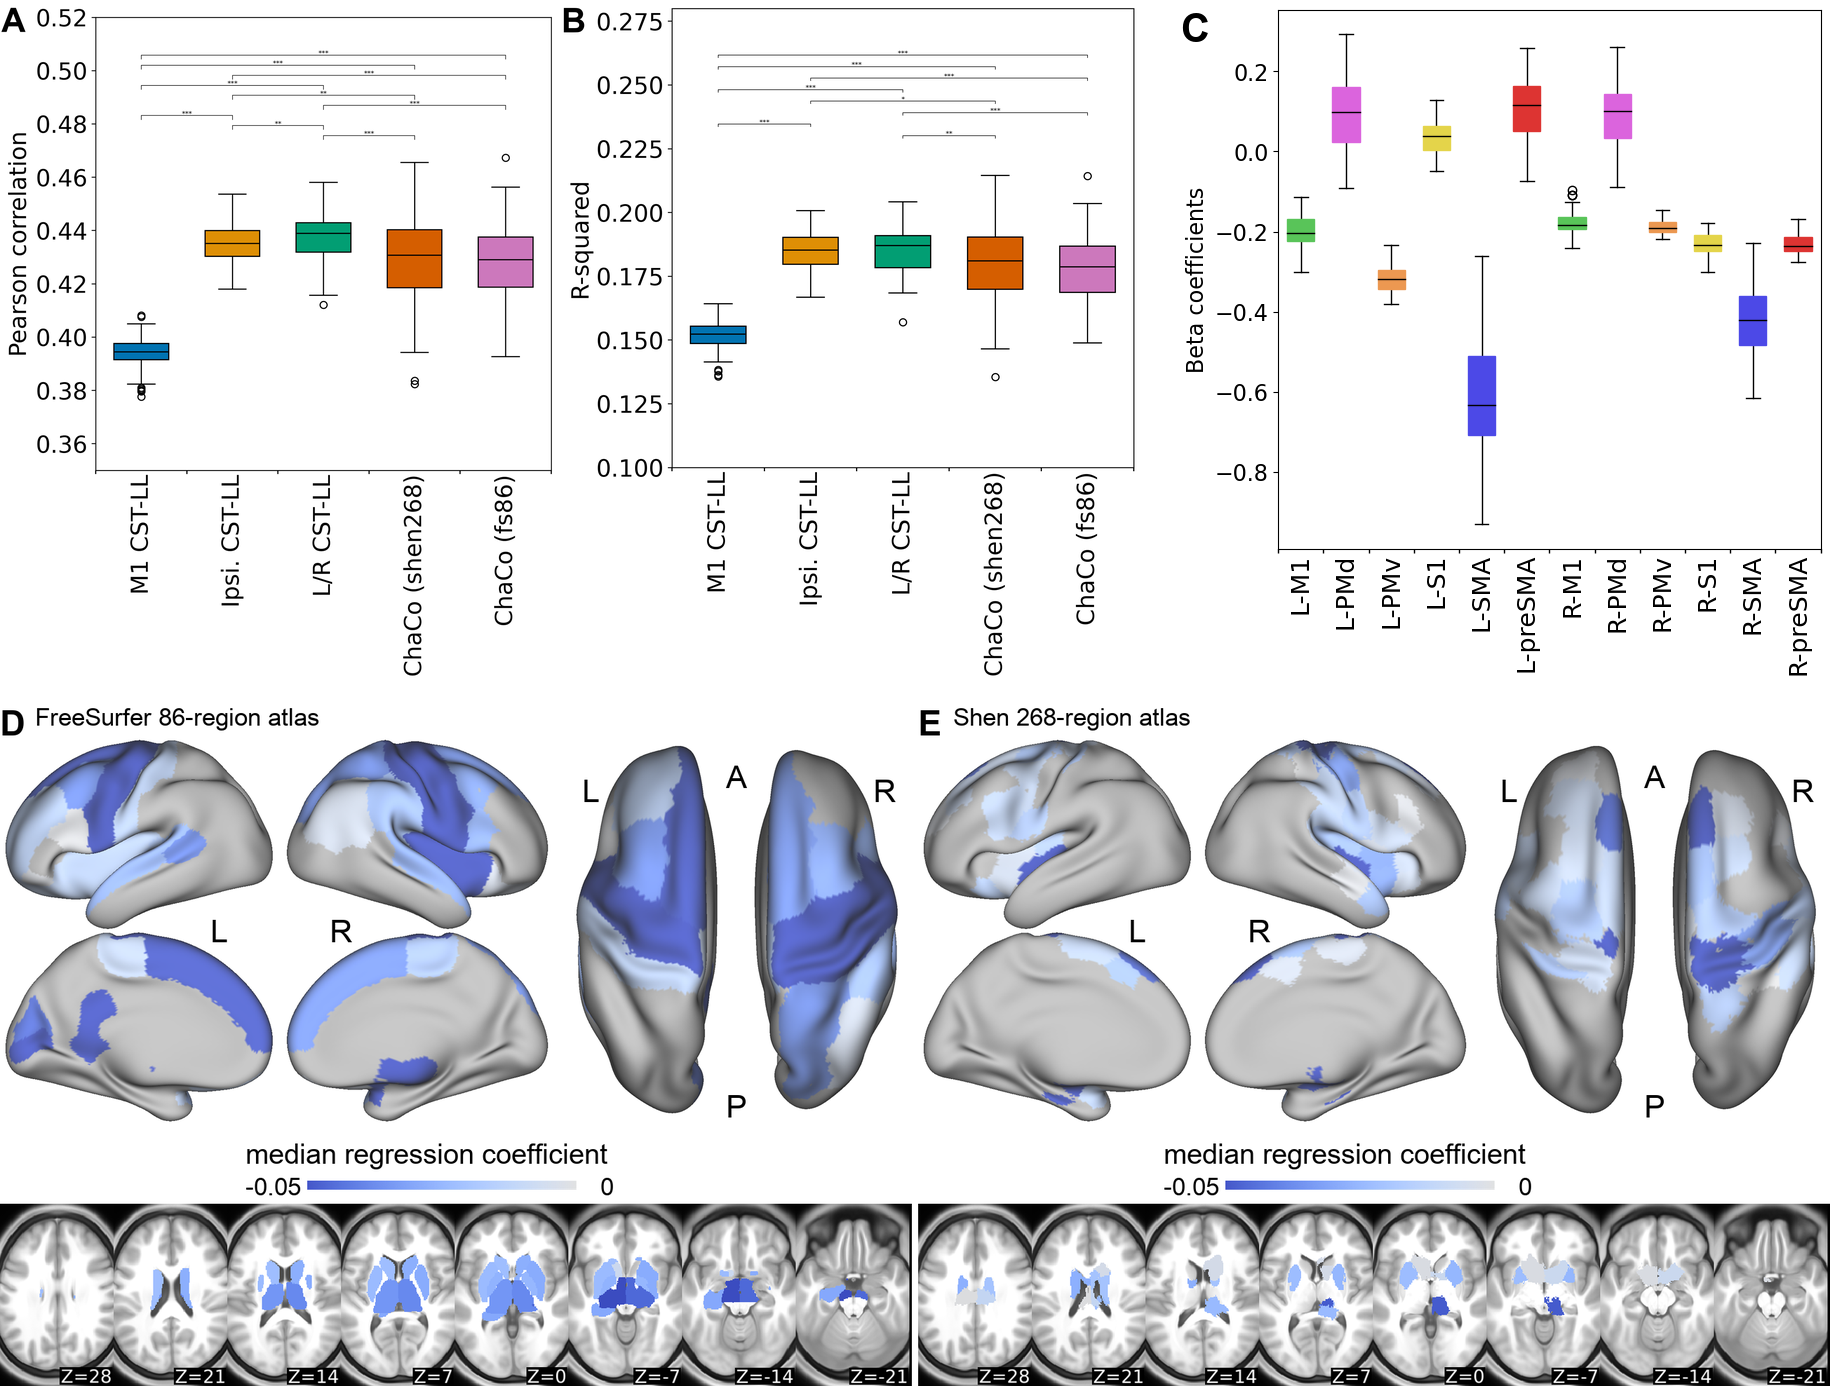
\includegraphics[width=1\linewidth]{figures/Analysis1.png}
\caption{Summary of model performance metrics across all models tested and feature weights (regression coefficients) for best-performing models.  \textbf{A.} and \textbf{B.} Distribution of model performance (mean Pearson correlation/$R^2$ across 5 outer folds for 100 permutations of the data).  Boxplots are colored abritrarily for clarity and are plotted in similarly-colored pairs to indicate performance using the full training data ("Acute $\Plus$  chronic") versus only chronic data ("Chronic only"). The boxes extend from the lower to upper quartile values of the data, with a line at the median. Whiskers represent the range of the data from [Q1-1.5*IQR, Q3+1.5*IQR].
\textbf{C.} and \textbf{D.} Average negative feature weights for the top 2 best-performing models (fs86-ChaCo without feature selection, shen268-ChaCo with feature selection, respectively). For fs86-ChaCo (left), displaying mean regression coefficients across 100 permutations. For shen268-ChaCo (right), displaying mean regression coefficients for regions that were selected in at least half of the models (i.e., were included in the model in at least 250/500 outer folds). }
\label{analysis1}
\end{figure}




\begin{figure}[htp]
\centering
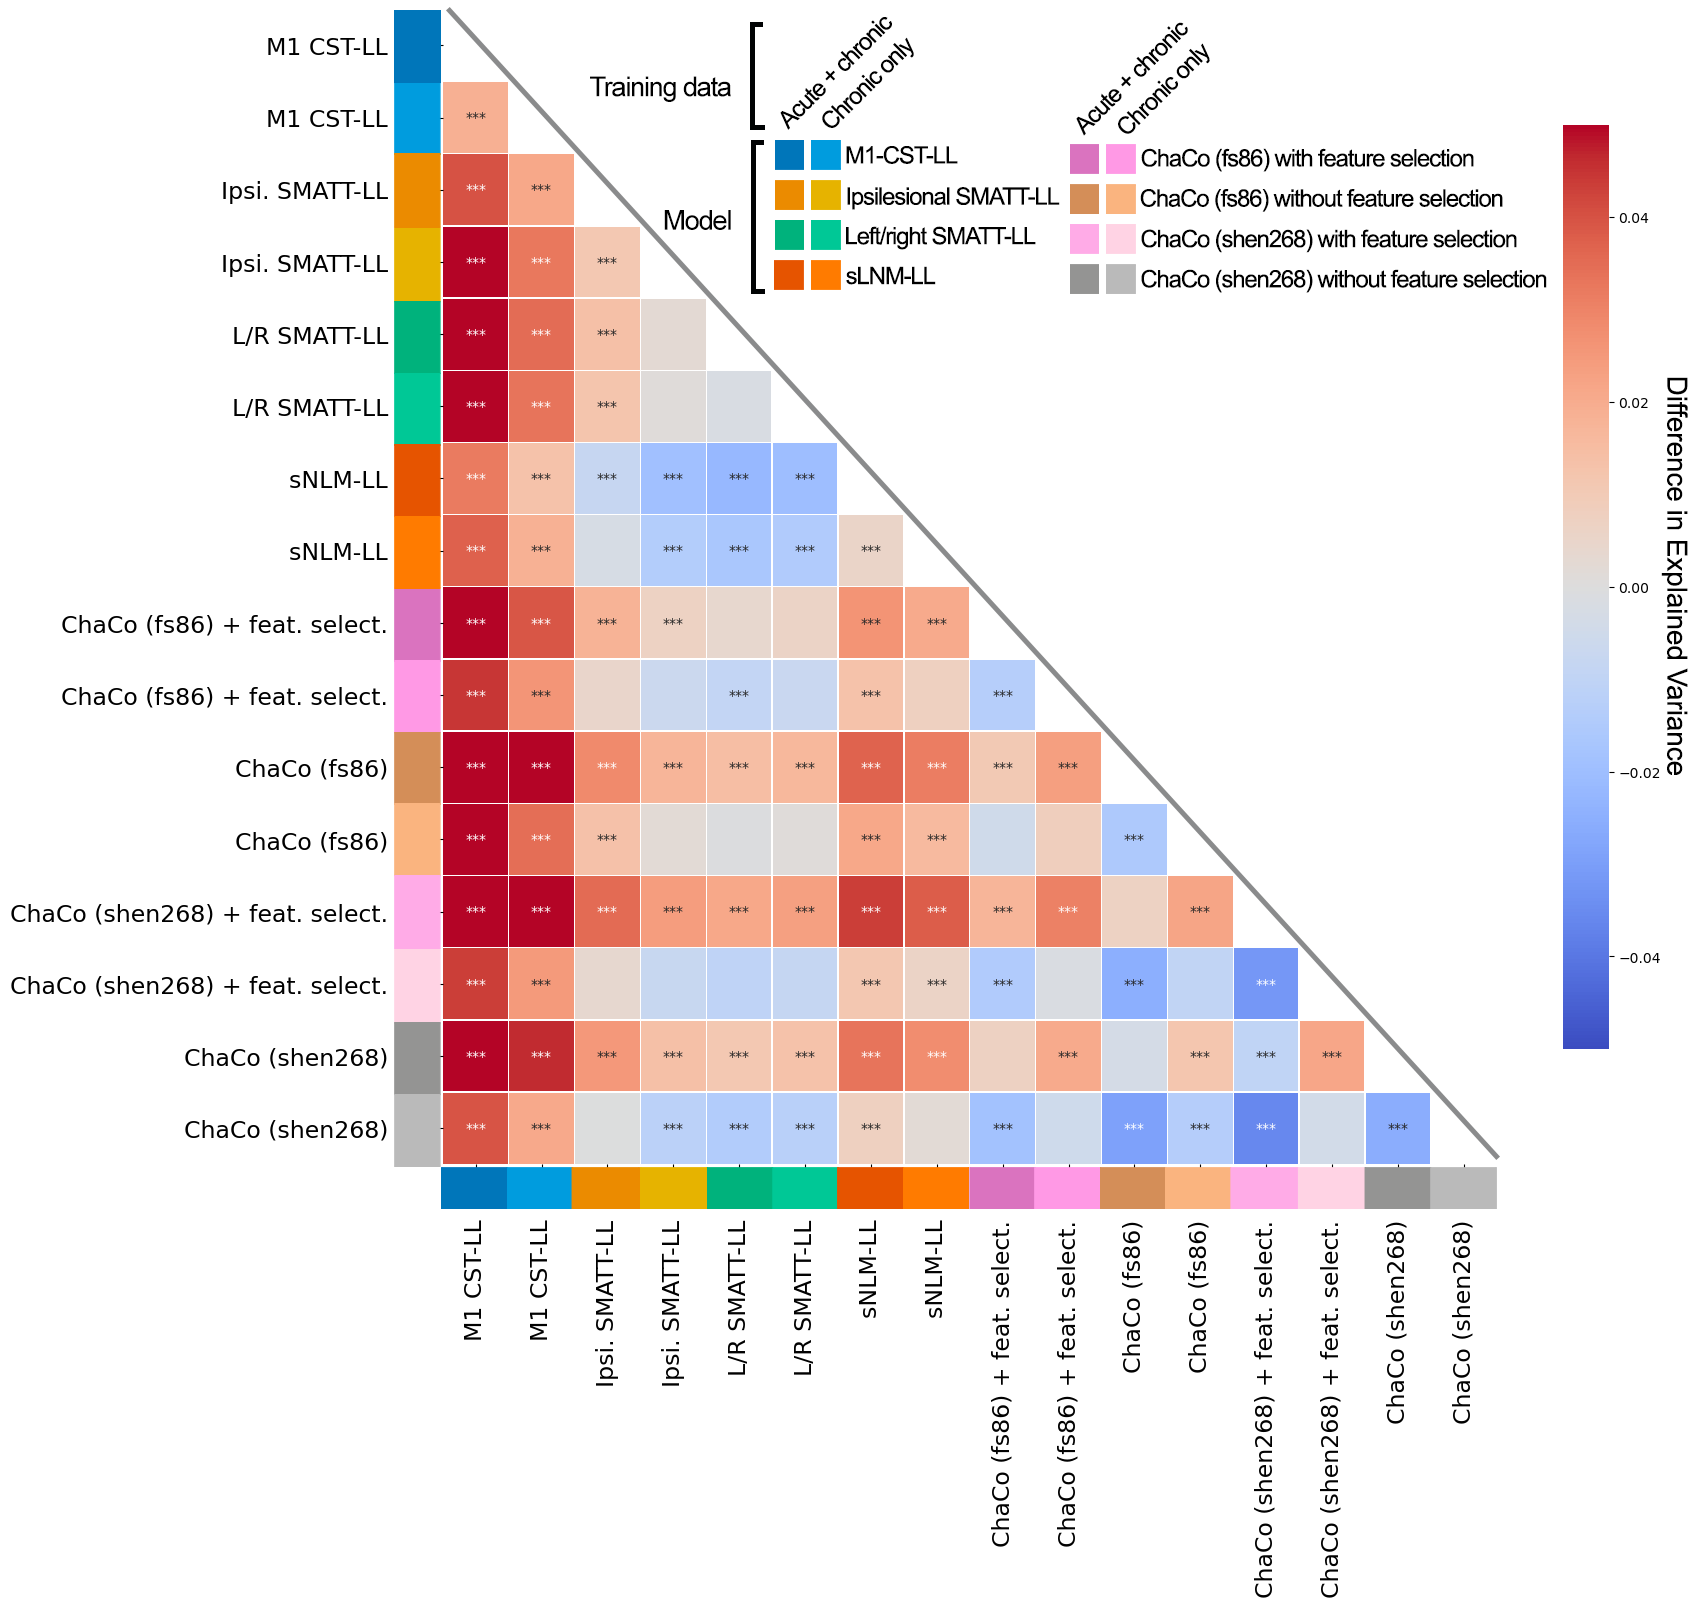
\includegraphics[width=1\linewidth]{figures/analysis_1_matrix_figure_colors.png}
\caption{Differences in model performance for prediction of normalized motor scores. Difference in explained variance between pairs of models using different lesion metrics and different training data. Model differences were calculated by averaging the difference in explained variance for each of the 100 train/test splits. Significance of differences in explained variance were evaluated using exact tests for differences. $***$ denotes corrected $p < 0.001$, $**$ denotes corrected $p < 0.01$, $*$ denotes corrected $p < 0.05$ after Bonferroni correction. A positive difference value indicates that the model on the y-axis (vertical) has a greater explained variance than the model on the x-axis (horizontal).
 }
\label{analysis1}
\end{figure}

\begin{figure}[htp]
\centering
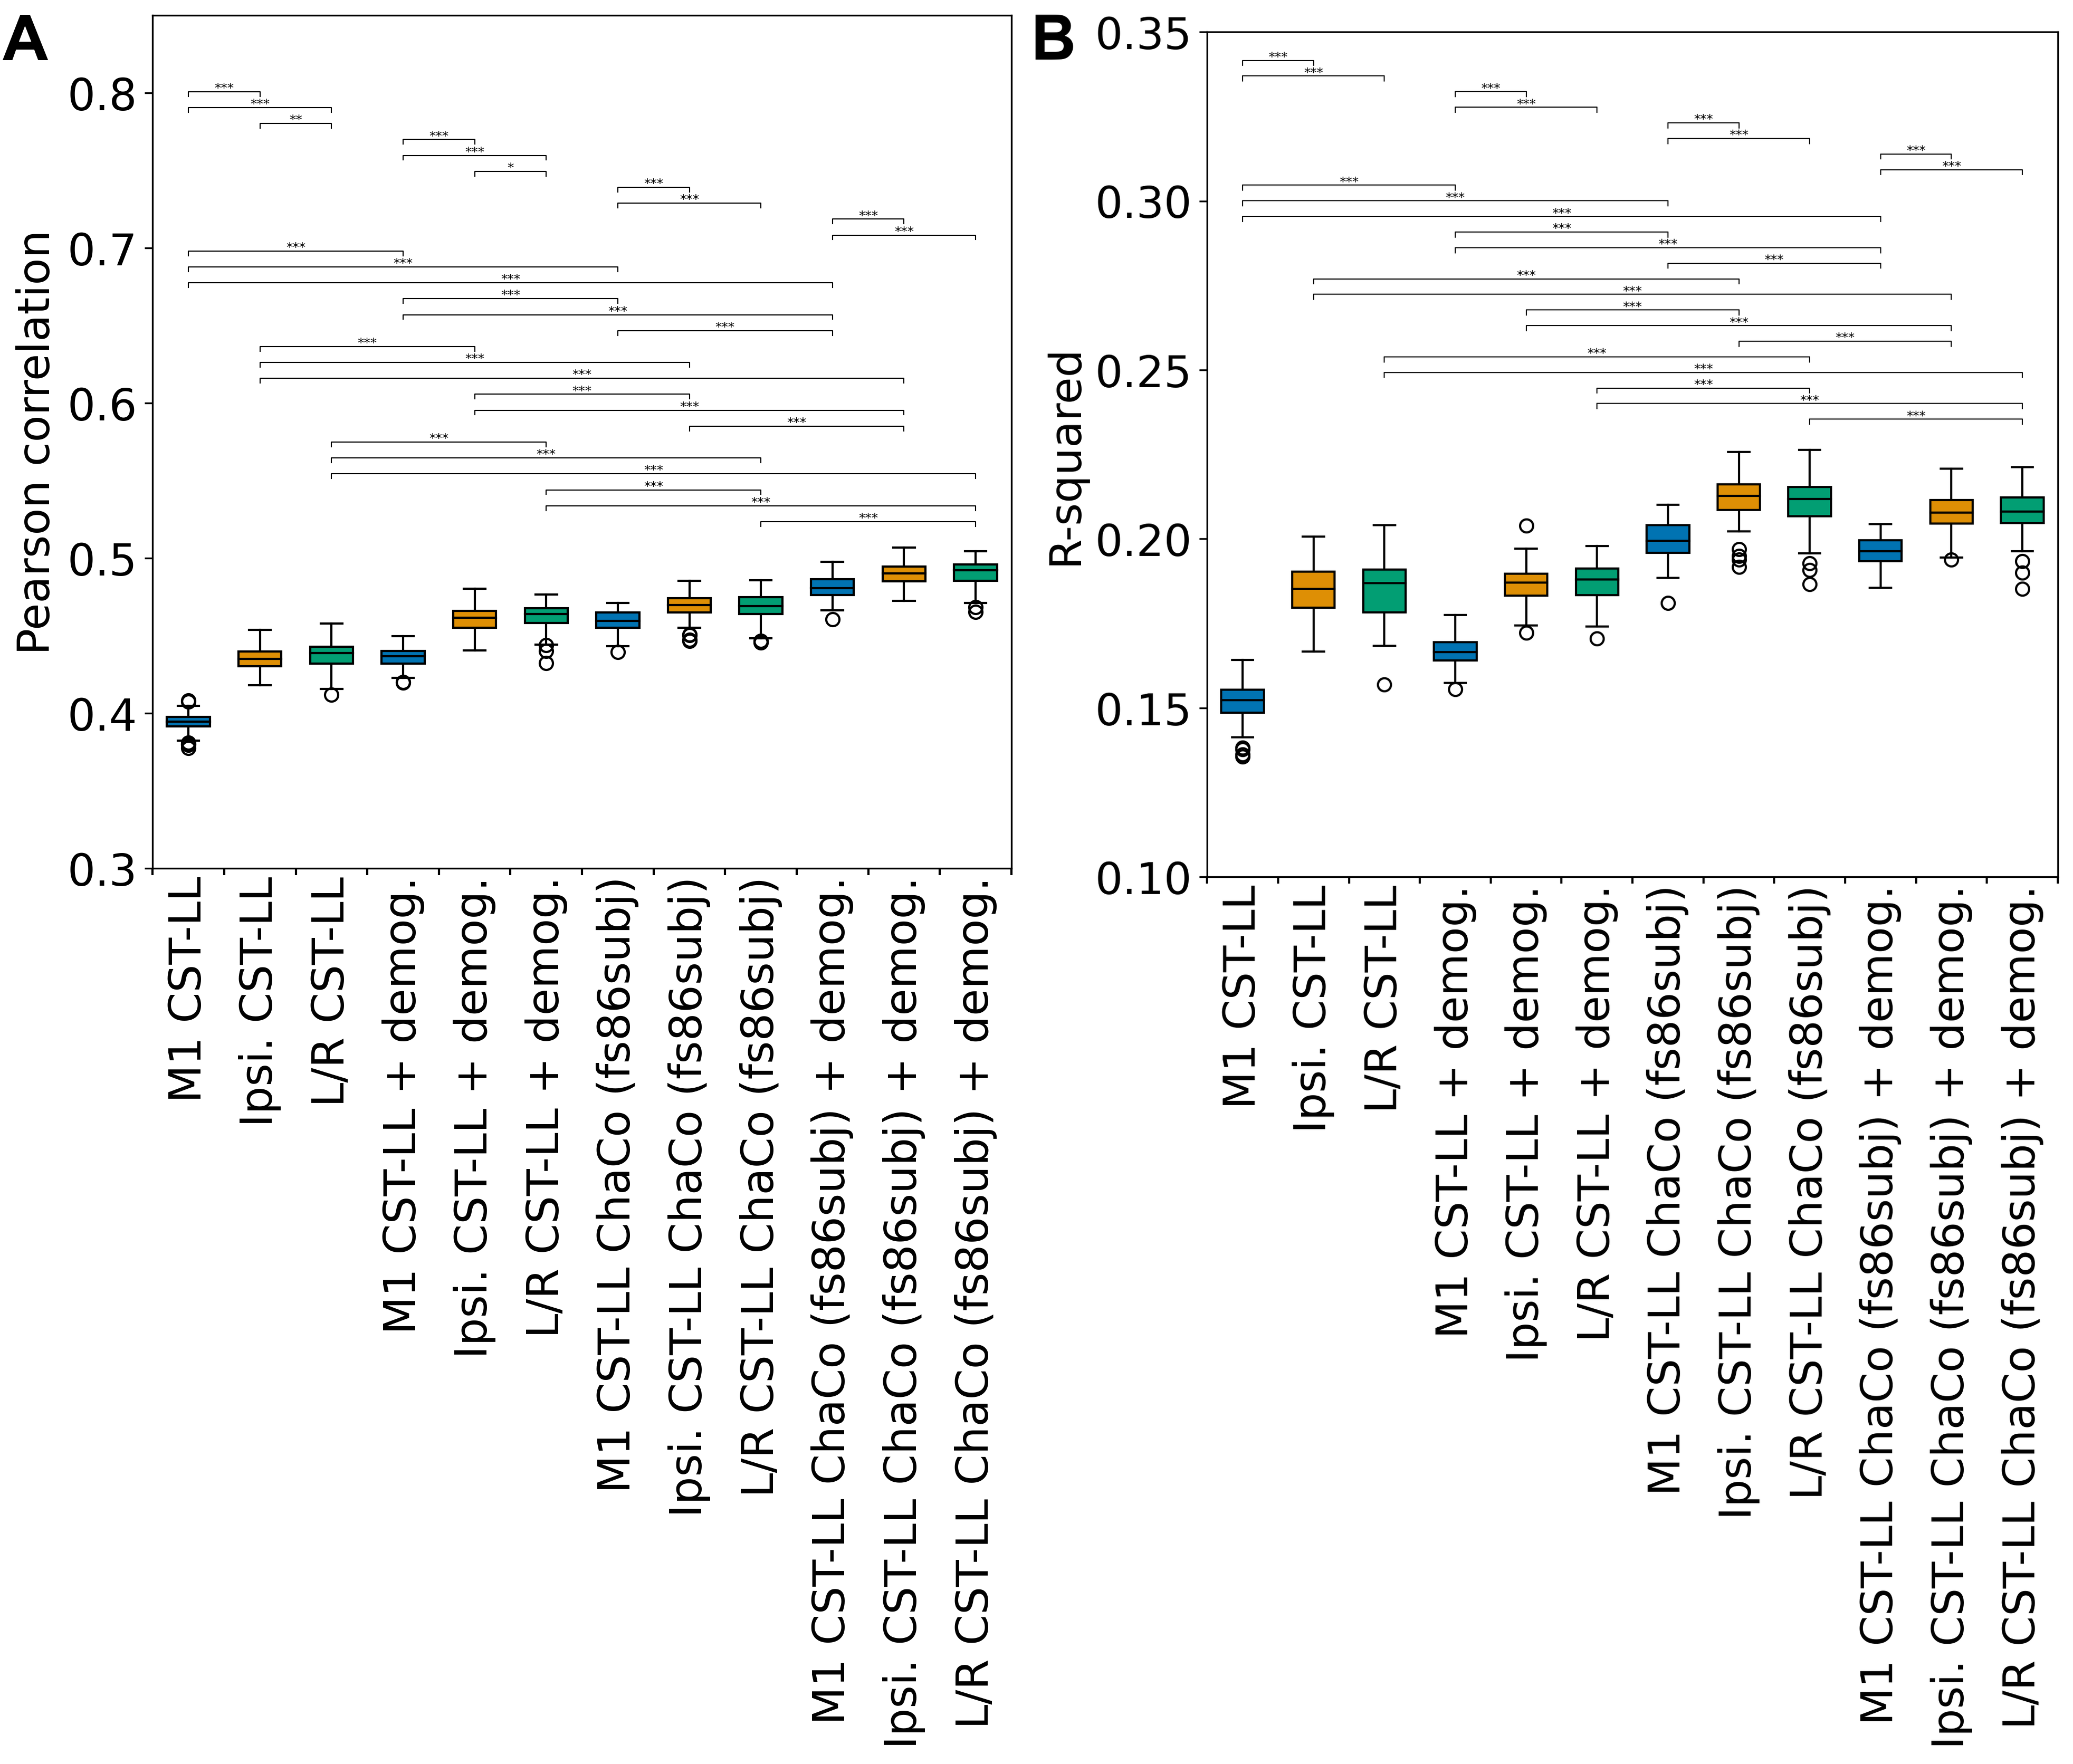
\includegraphics[width=1\linewidth]{figures/Analysis2.png}
\caption{Ensemble model results. coefficients and model performance using Group KFold cross-validation (test/validate on independent imaging site). \textbf{A.} and \textbf{B.} display regression coefficients for regional ChaCo scores (FreeSurfer 86-region atlas, and Shen268-region atlas, respectively). Average feature weights for regions that were selected in at least half of the models (i.e., were included in the model in at least 250/500 outer folds). \textbf{C.} Sensorimotor area tract template feature importance for analysis 2. Includes primary motor cortex (M1), dorsal premotor cortex (PMd), ventral premotor cortex (PMv), supplementary motor area (SMA), pre-supplementary motor area (pre-SMA), primary sensory cortex (S1).}
\label{nemotool}
\end{figure}



\section{Discussion}

\clearpage



\printbibliography
\section*{Supplementary Results}

\beginsupplement
\begin{figure}[ht]
\centering
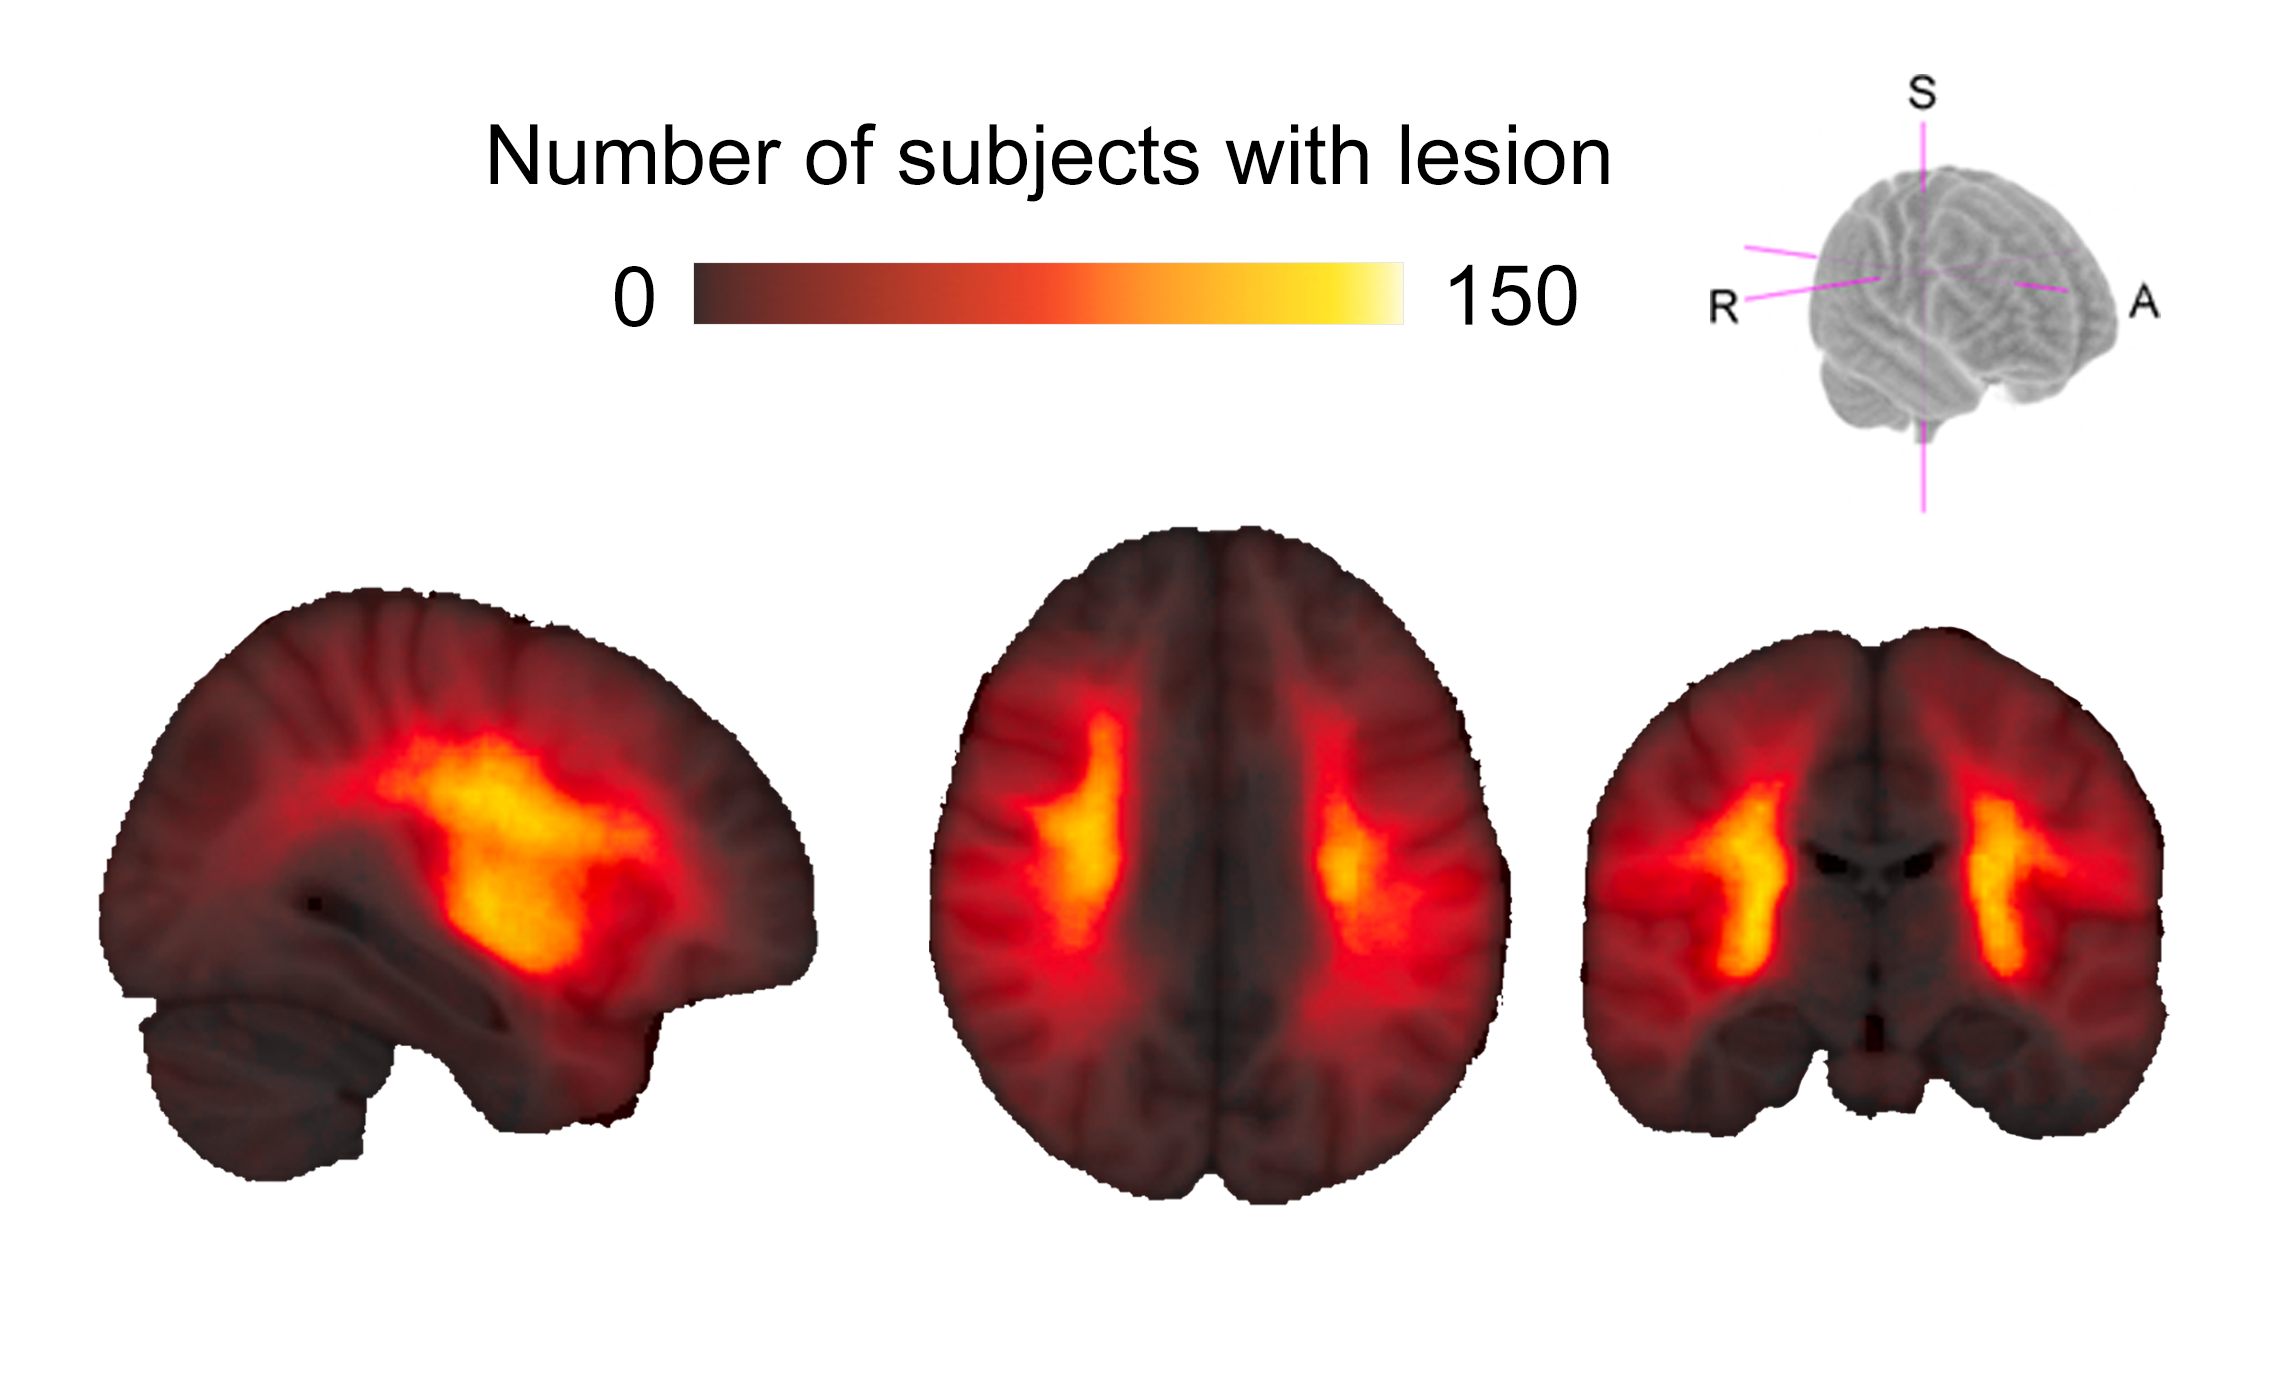
\includegraphics[width=0.8\linewidth]{figures/distribution_lesions.png}
\caption{Distribution of lesions in ENIGMA cohort.}
\label{lesiondist}
\end{figure}


\begin{table}[h]
\centering
\caption{Number of subjects with data for each type of assessment, broken down by chronicity (acute/chronic) and site. FMA UE = Fugl Meyer Assessment of Upper Extremity [0-66], Barthel = Barthel Index [0-100], NIHSS (National Institutes of Health Stroke Score) [0-42], ARAT = Action Research Arm Test [0-57]}
\label{motor_scores}
\begin{tabular}{lrlllllll}
\toprule
 & Total N. & FMA-UE  & Barthel & NIHSS  & ARAT \\
 & & &  &  \\
 \textbf{Acute}  & & & & & \\
\arrayrulecolor{black!30}\midrule
r005 & 1 & 1 & 0 & 0 & 0 \\
r009 & 50 & 0 & 0 & 50 & 0 \\
r025 & 9 & 9 & 0 & 0 & 0 \\
r028 & 1 & 1 & 0 & 0 & 0 \\
r031 & 36 & 36 & 0 & 0 & 0 \\
r038 & 72 & 0 & 72 & 0 & 0 \\
r040 & 57 & 0 & 57 & 0 & 0 \\
r047 & 2 & 2 & 0 & 0 & 0 \\
r049 & 21 & 0 & 0 & 21 & 0 \\
r050 & 14 & 0 & 0 & 14 & 0 \\
r053 & 52 & 0 & 0 & 52 & 0 \\
r054 & 12 & 12 & 0 & 0 & 0 \\

& & & & & \\
 \textbf{Chronic}  & & & & & \\
\arrayrulecolor{black!30}\midrule
r001 & 39 & 39 & 0 & 0 & 0 \\
r002 & 12 & 12 & 0 & 0 & 0 \\
r003 & 15 & 15 & 0 & 0 & 0 \\
r004 & 19 & 19 & 0 & 0 & 0 \\
r005 & 27 & 27 & 0 & 0 & 0 \\
r009 & 60 & 0 & 0 & 60 & 0 \\
r025 & 16 & 16 & 0 & 0 & 0 \\
r027 & 28 & 28 & 0 & 0 & 0 \\
r028 & 21 & 21 & 0 & 0 & 0 \\
r031 & 1 & 1 & 0 & 0 & 0 \\
r034 & 15 & 15 & 0 & 0 & 0 \\
r035 & 15 & 15 & 0 & 0 & 0 \\
r038 & 18 & 0 & 18 & 0 & 0 \\
r040 & 14 & 0 & 14 & 0 & 0 \\
r042 & 22 & 22 & 0 & 0 & 0 \\
r044 & 4 & 4 & 0 & 0 & 0 \\
r045 & 4 & 4 & 0 & 0 & 0 \\
r046 & 11 & 11 & 0 & 0 & 0 \\
r047 & 44 & 44 & 0 & 0 & 0 \\
r048 & 43 & 43 & 0 & 0 & 0 \\
r052 & 32 & 32 & 0 & 0 & 0 \\
r053 & 2 & 0 & 0 & 2 & 0 \\
\bottomrule
\end{tabular}
\end{table}


\begin{figure}
\begin{subfigure}{0.5\textwidth}
  \centering
  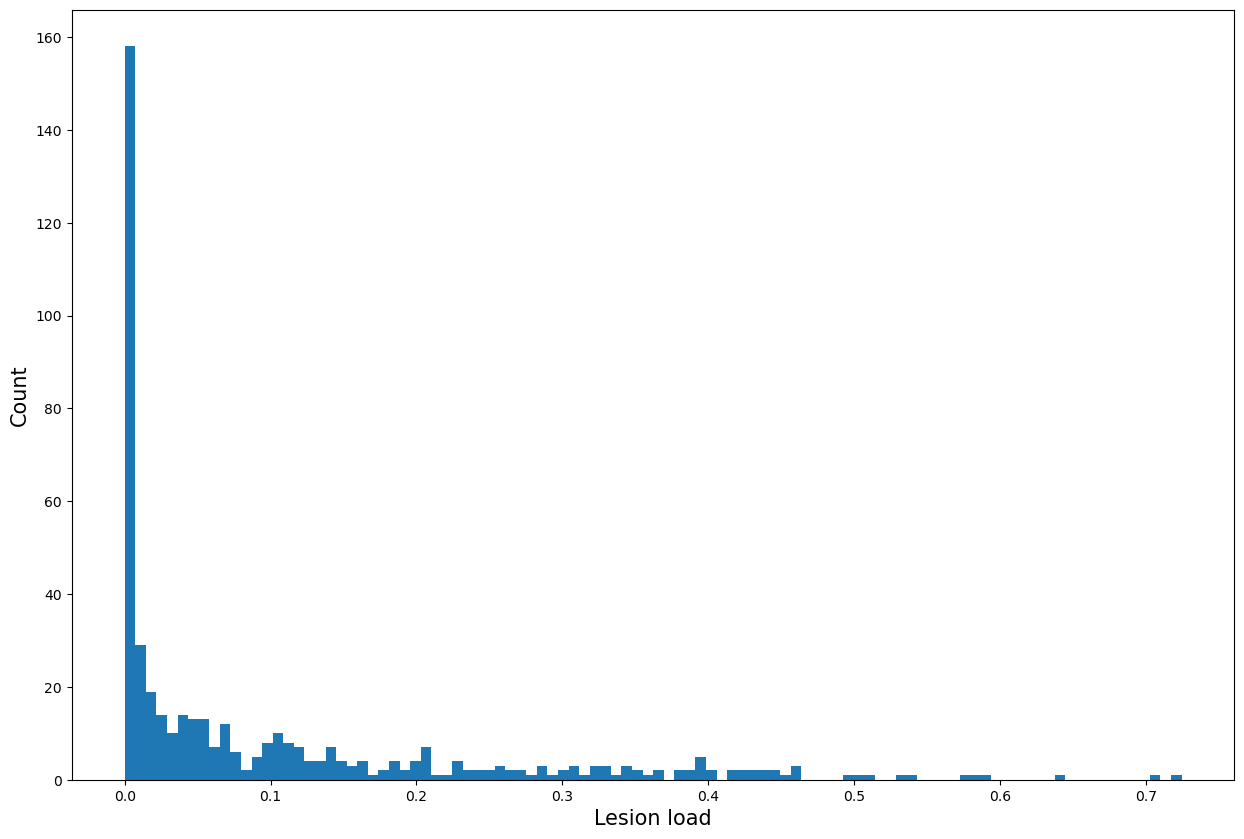
\includegraphics[width=1\linewidth]{figures/m1_lesionload.png}
  \caption{M1-CST lesion load distribution.}
  \label{fig:sfig1}
\end{subfigure}
\begin{subfigure}{0.5\textwidth}
  \centering
  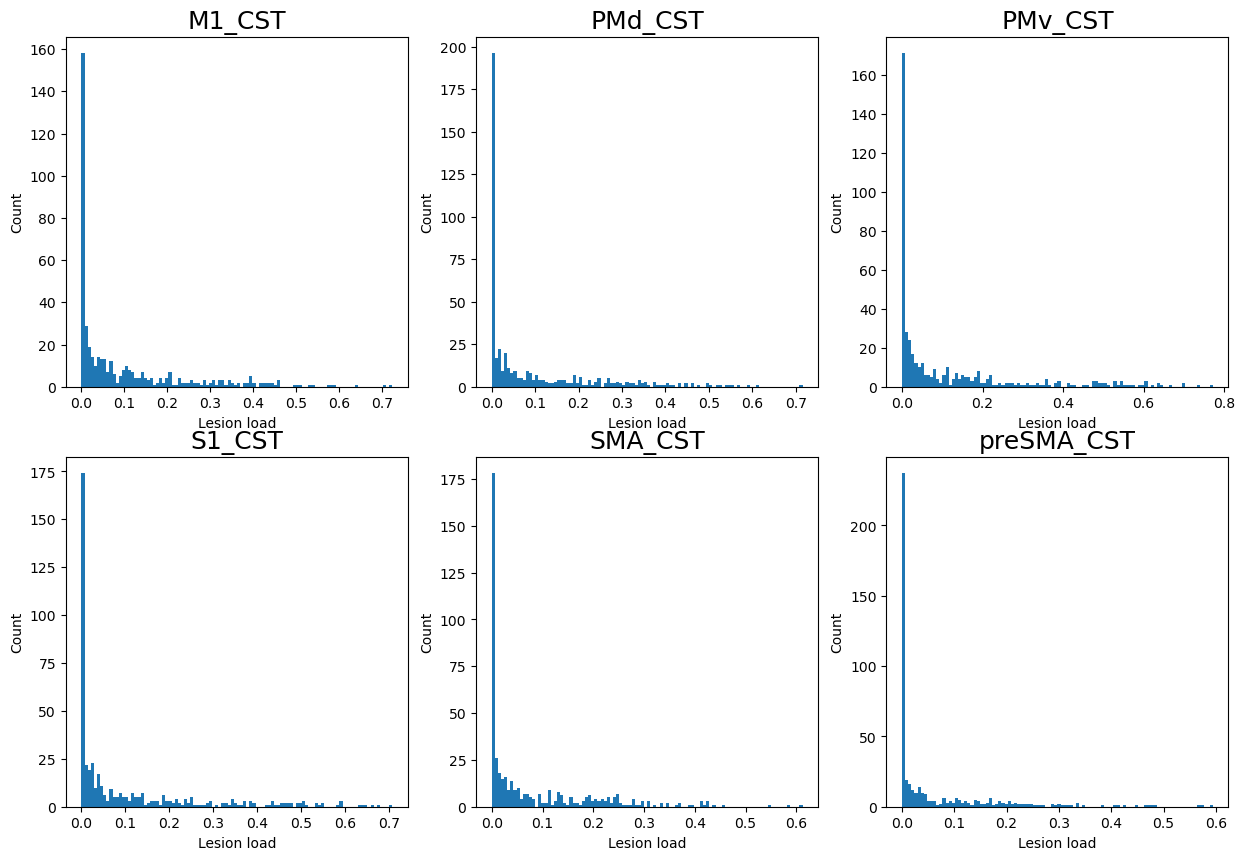
\includegraphics[width=1\linewidth]{figures/all_lesionload.png}
  \caption{Ipsilesional sensorimotor tract template (SMATT) lesion load distribution.}
  \label{fig:sfig2}
\end{subfigure}
\begin{subfigure}{1\textwidth}
  \centering
  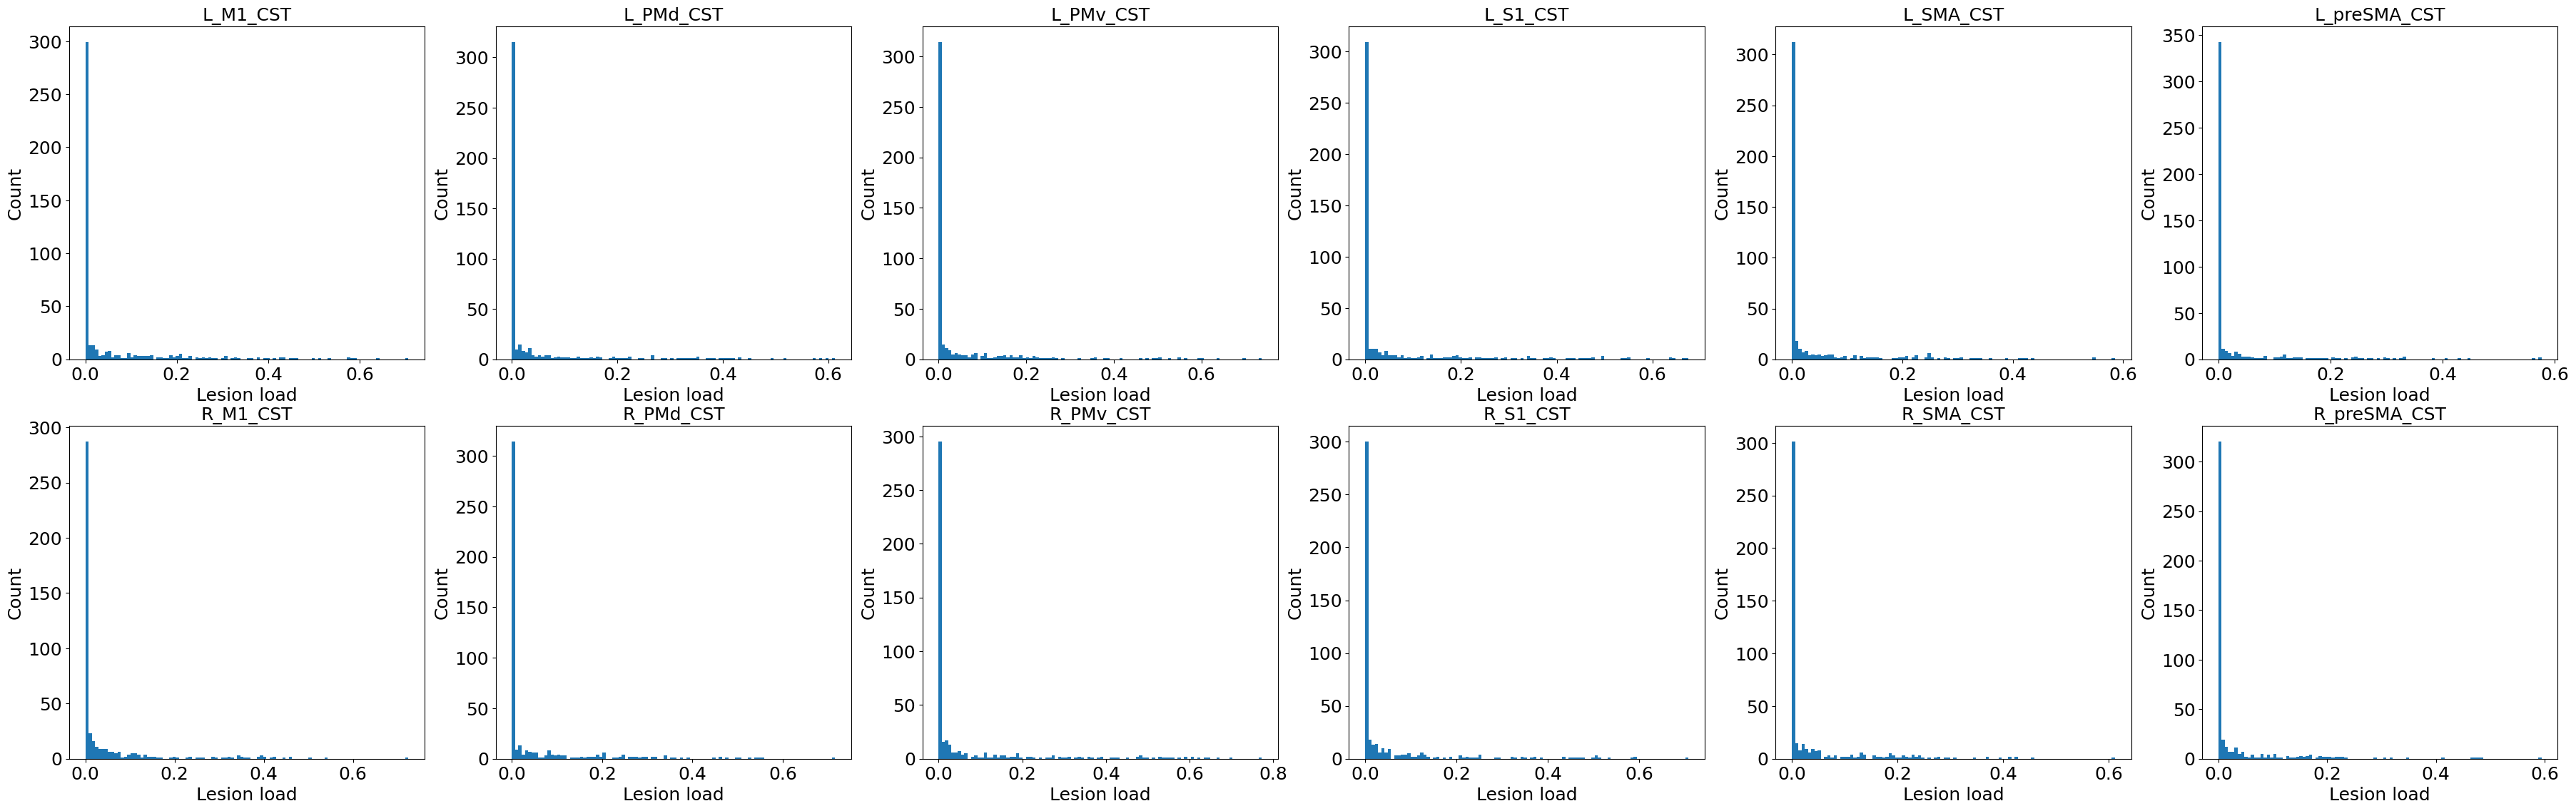
\includegraphics[width=1\linewidth]{figures/all2h_lesionload.png}
  \caption{Left and right hemisphere sensorimotor tract template (SMATT) lesion load distribution.}
  \label{fig:sfig2}
\end{subfigure}
\caption{Distribution of lesion load variables for chronic subjects.}
\label{lesion_load_dist}
\end{figure}


\begin{figure}[ht]
\centering
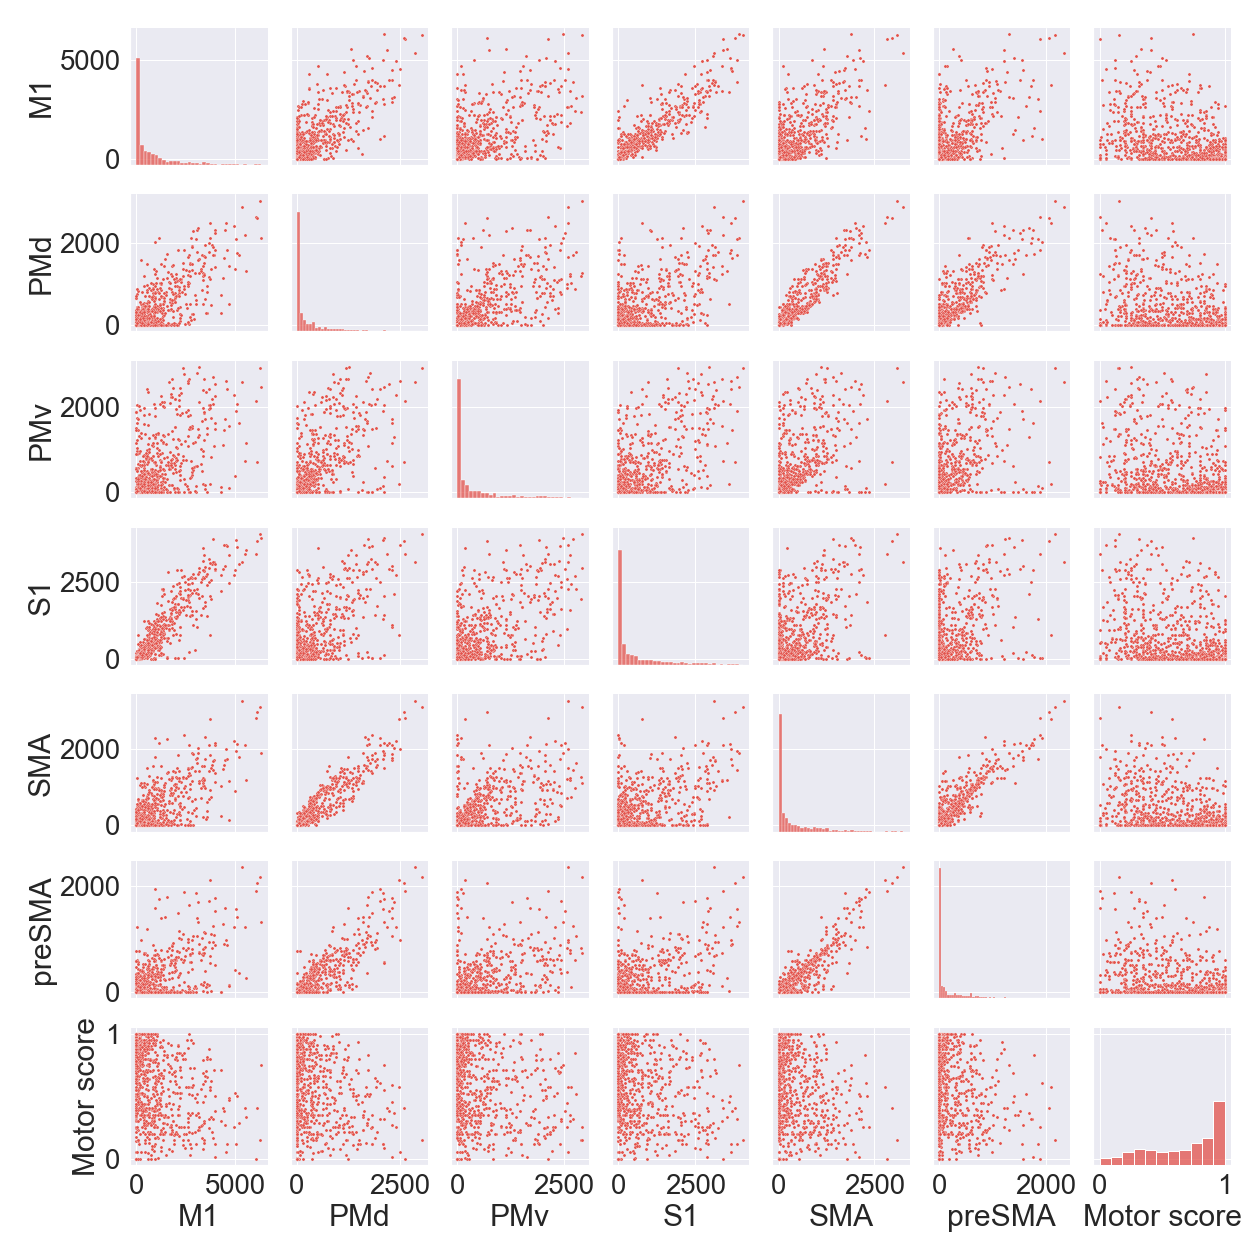
\includegraphics[width=0.8\linewidth]{figures/SMATT_scatterplts.png}
\caption{Correlations between lesion load calculated for each ipsilesional tract in the sensorimotor area tract template atlas.}
\label{smatt_pairwise_correlations}
\end{figure}

\begin{figure}[ht]
\centering
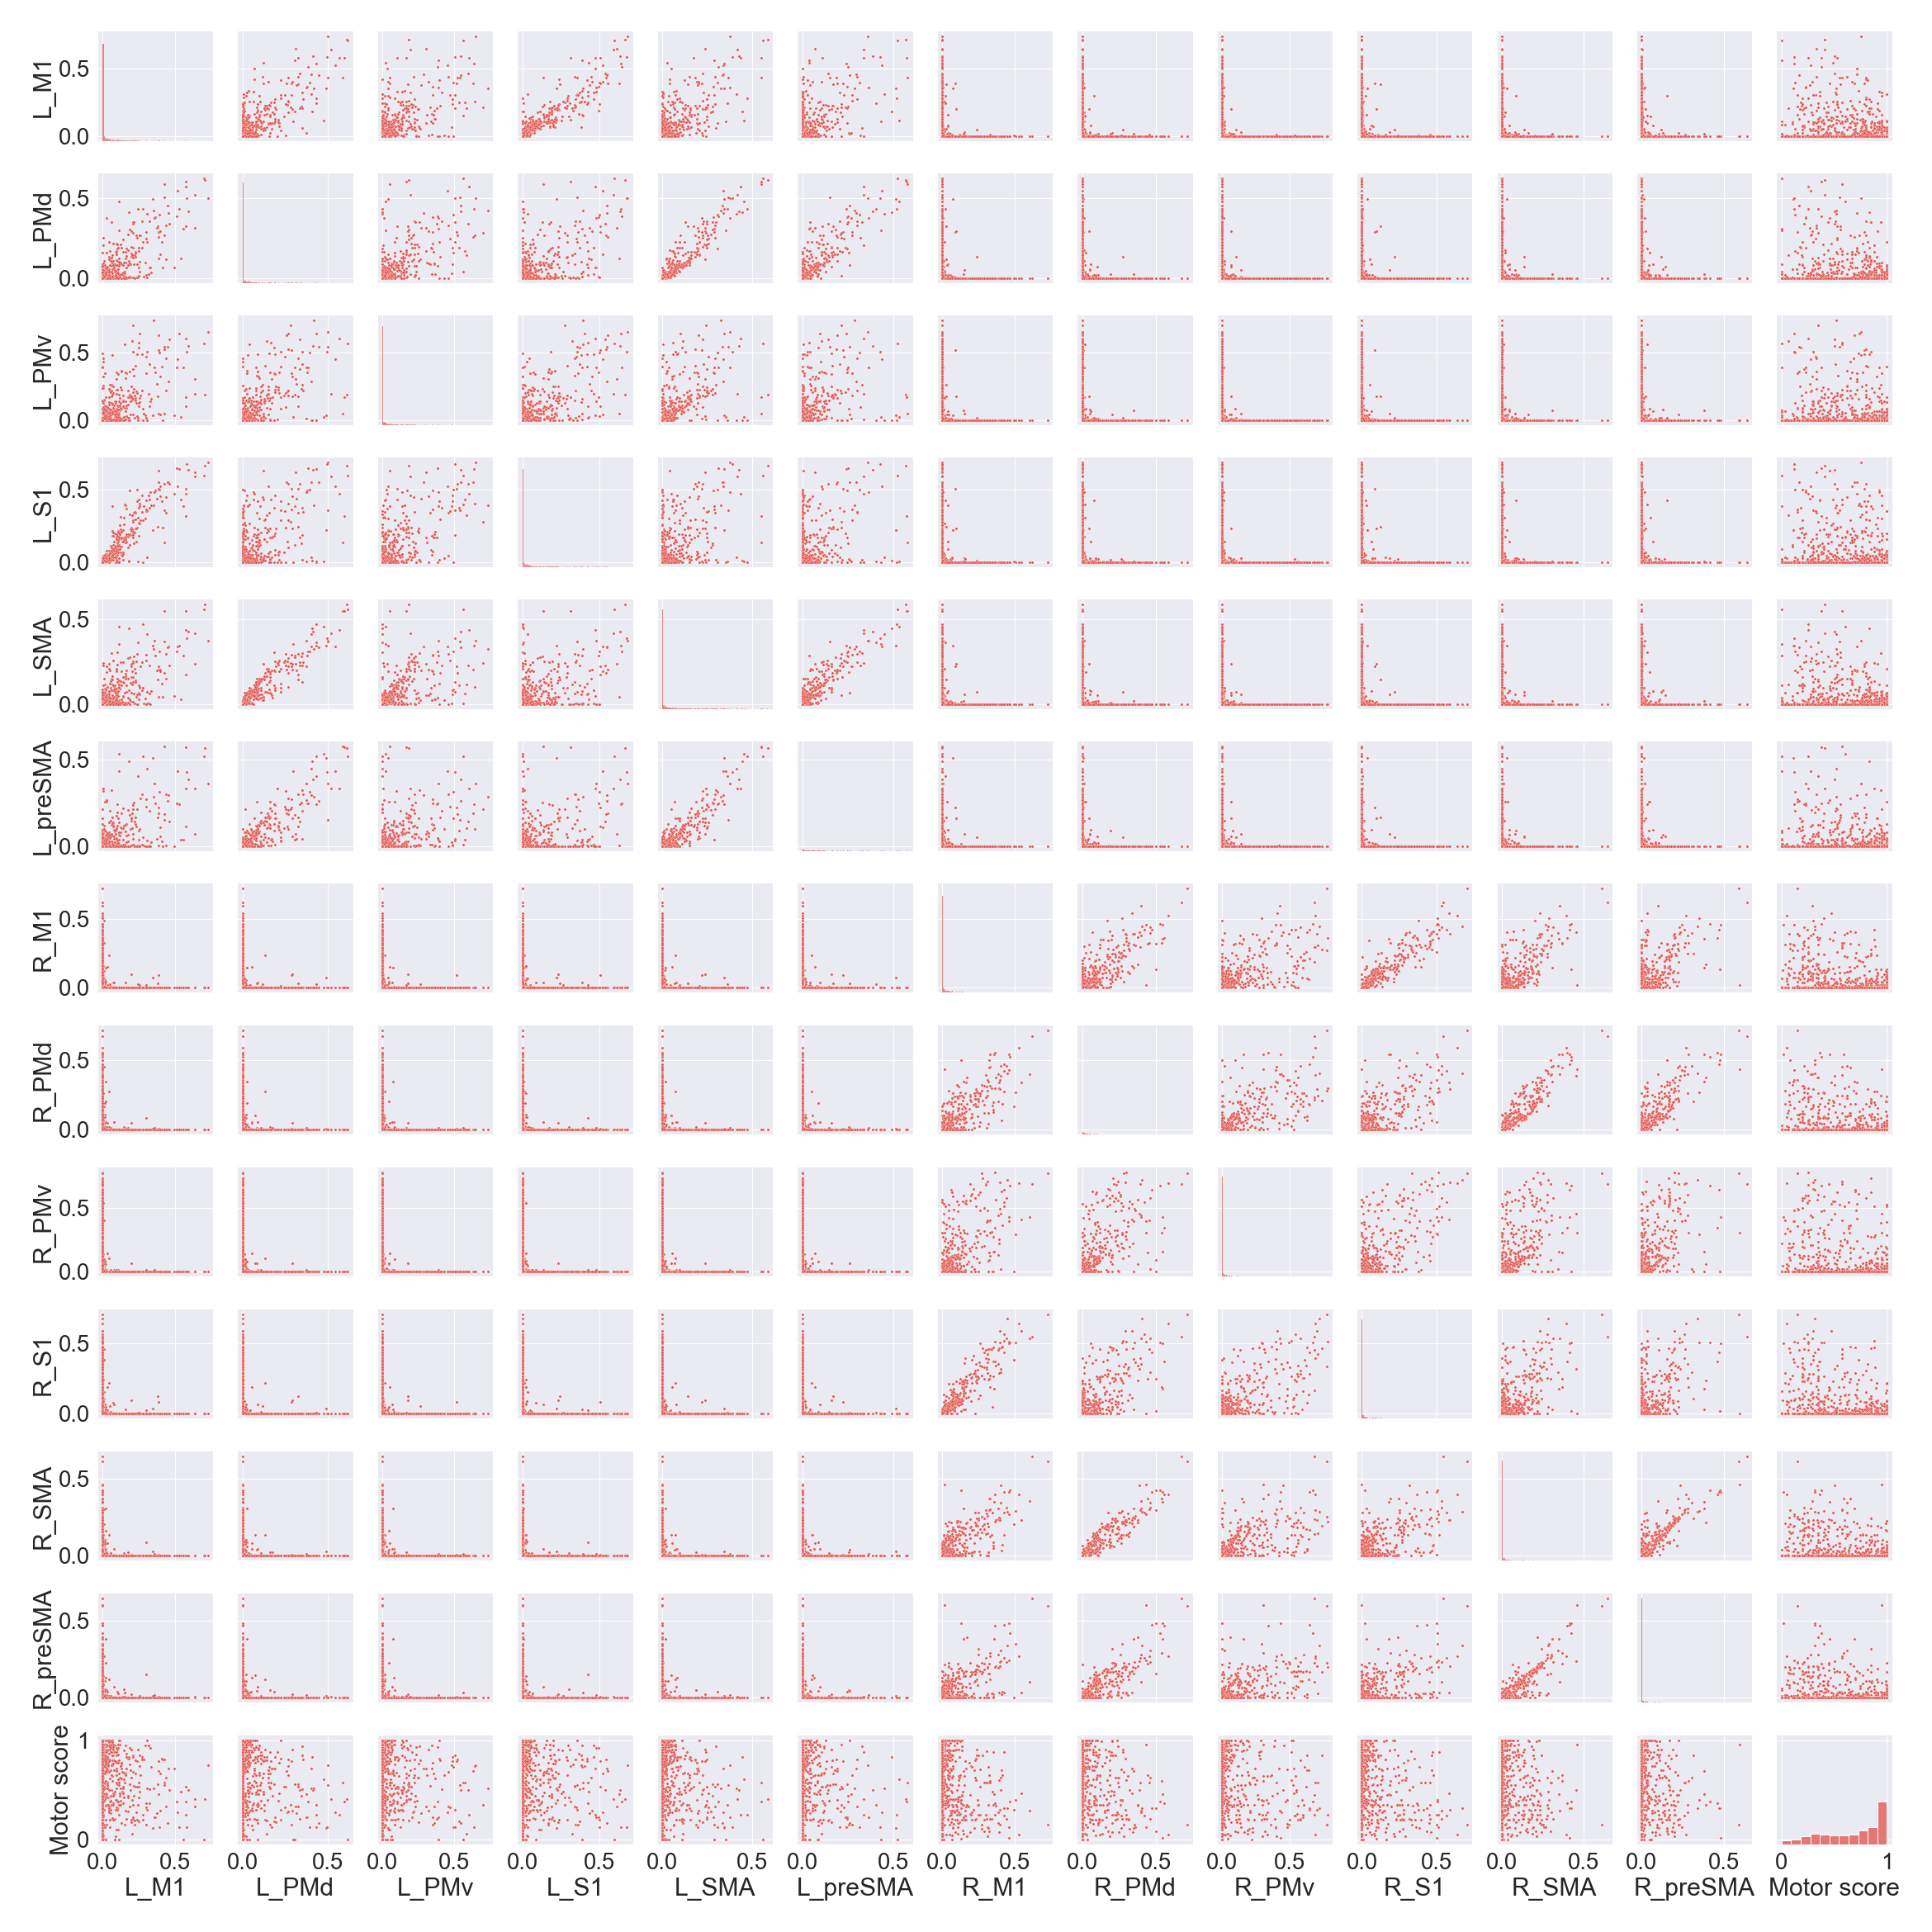
\includegraphics[width=1\linewidth]{figures/SMATT_bi_scatterplts.png}
\caption{Correlations between lesion load calculated for each left and right hemisphere tract in the sensorimotor area tract template atlas.}
\label{smatt_pairwise_correlations_bi}
\end{figure}

\begin{figure}[ht]
\centering
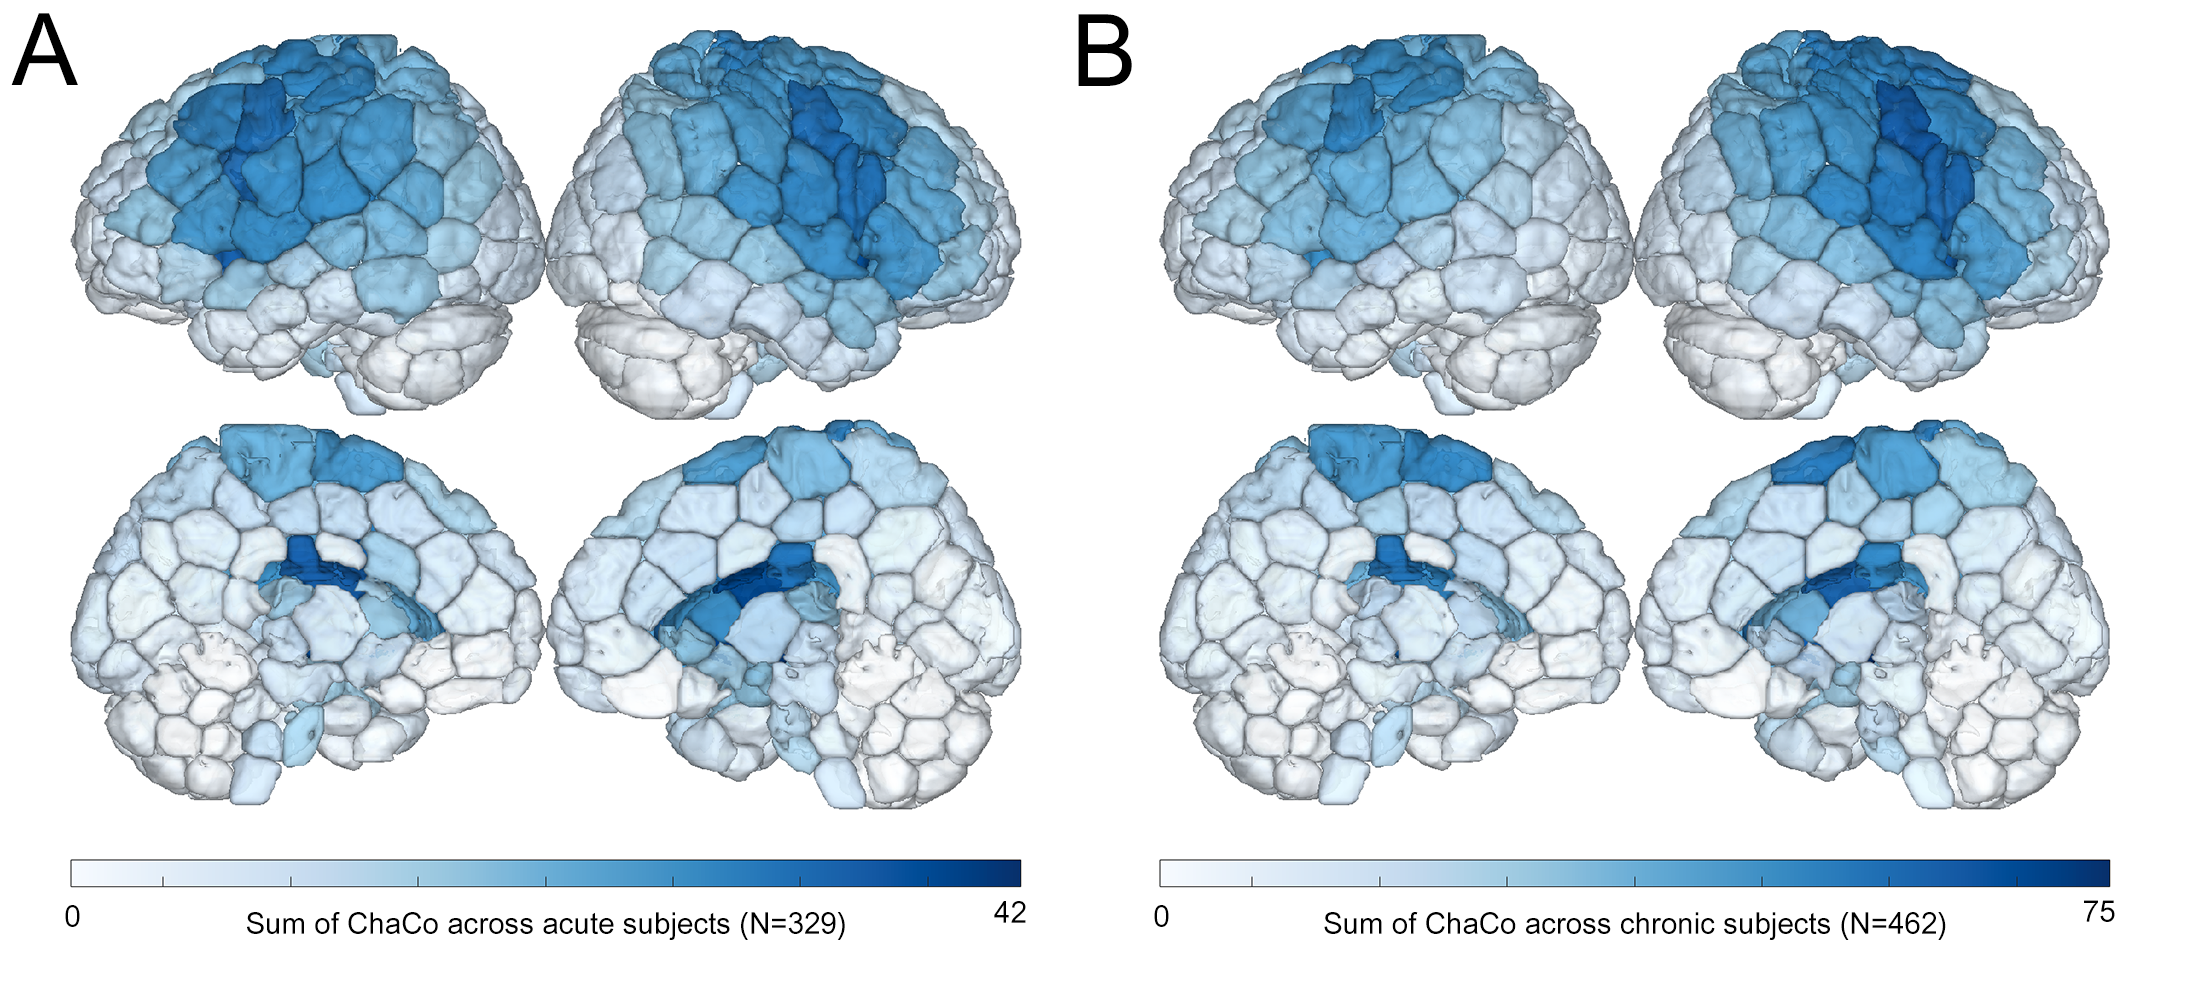
\includegraphics[width=0.8\linewidth]{figures/acutechronic_sumchaco.png}
\caption{Sum of regional change in connectivity (ChaCo) scores across subjects. Sum of ChaCo scores parcellated with the FreeSurfer 86-region atlas for acute (\textbf{A}) and chronic (\textbf{B}) subjects and for the Shen 268-region atlas for acute (\textbf{C}) and chronic (\textbf{D}) subjects.}
\label{sumchaco_acutechronic}
\end{figure}



\begin{figure}[ht]
\centering
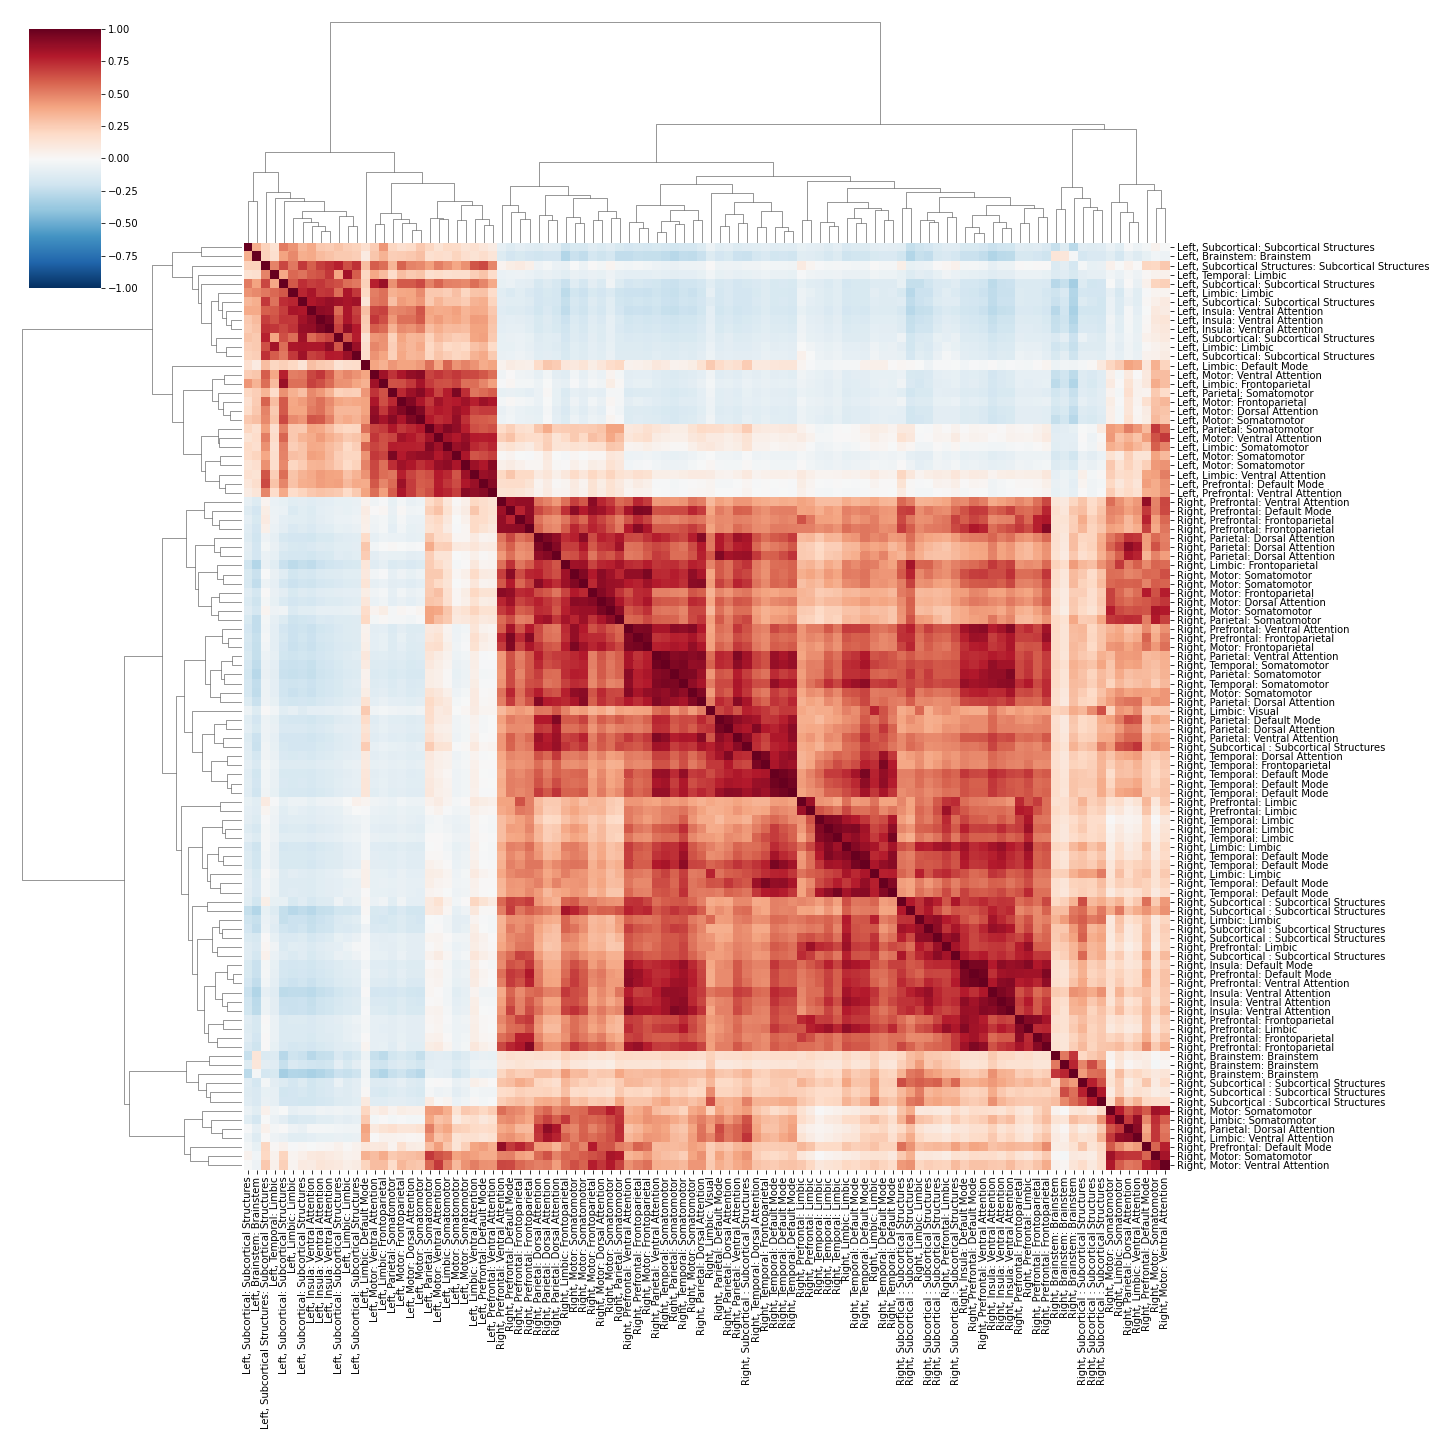
\includegraphics[width=1\linewidth]{figures/heatmap_shen268_correlation.png}
\caption{Hierarchically-clustered heatmap of the correlation matrix of the selected features (ChaCo scores) chosen in at least 50 percent of outer folds by correlation-based feature selection in ridge regression using the shen 268-region atlas. Heatmap (top left) displays values corresponding to correlation between features across subjects. Regions are labeled in the following format: "Hemisphere, lobe: Yeo Network".}
\label{heatmap_shen}
\end{figure}



\begin{figure}
\begin{subfigure}{0.5\textwidth}
  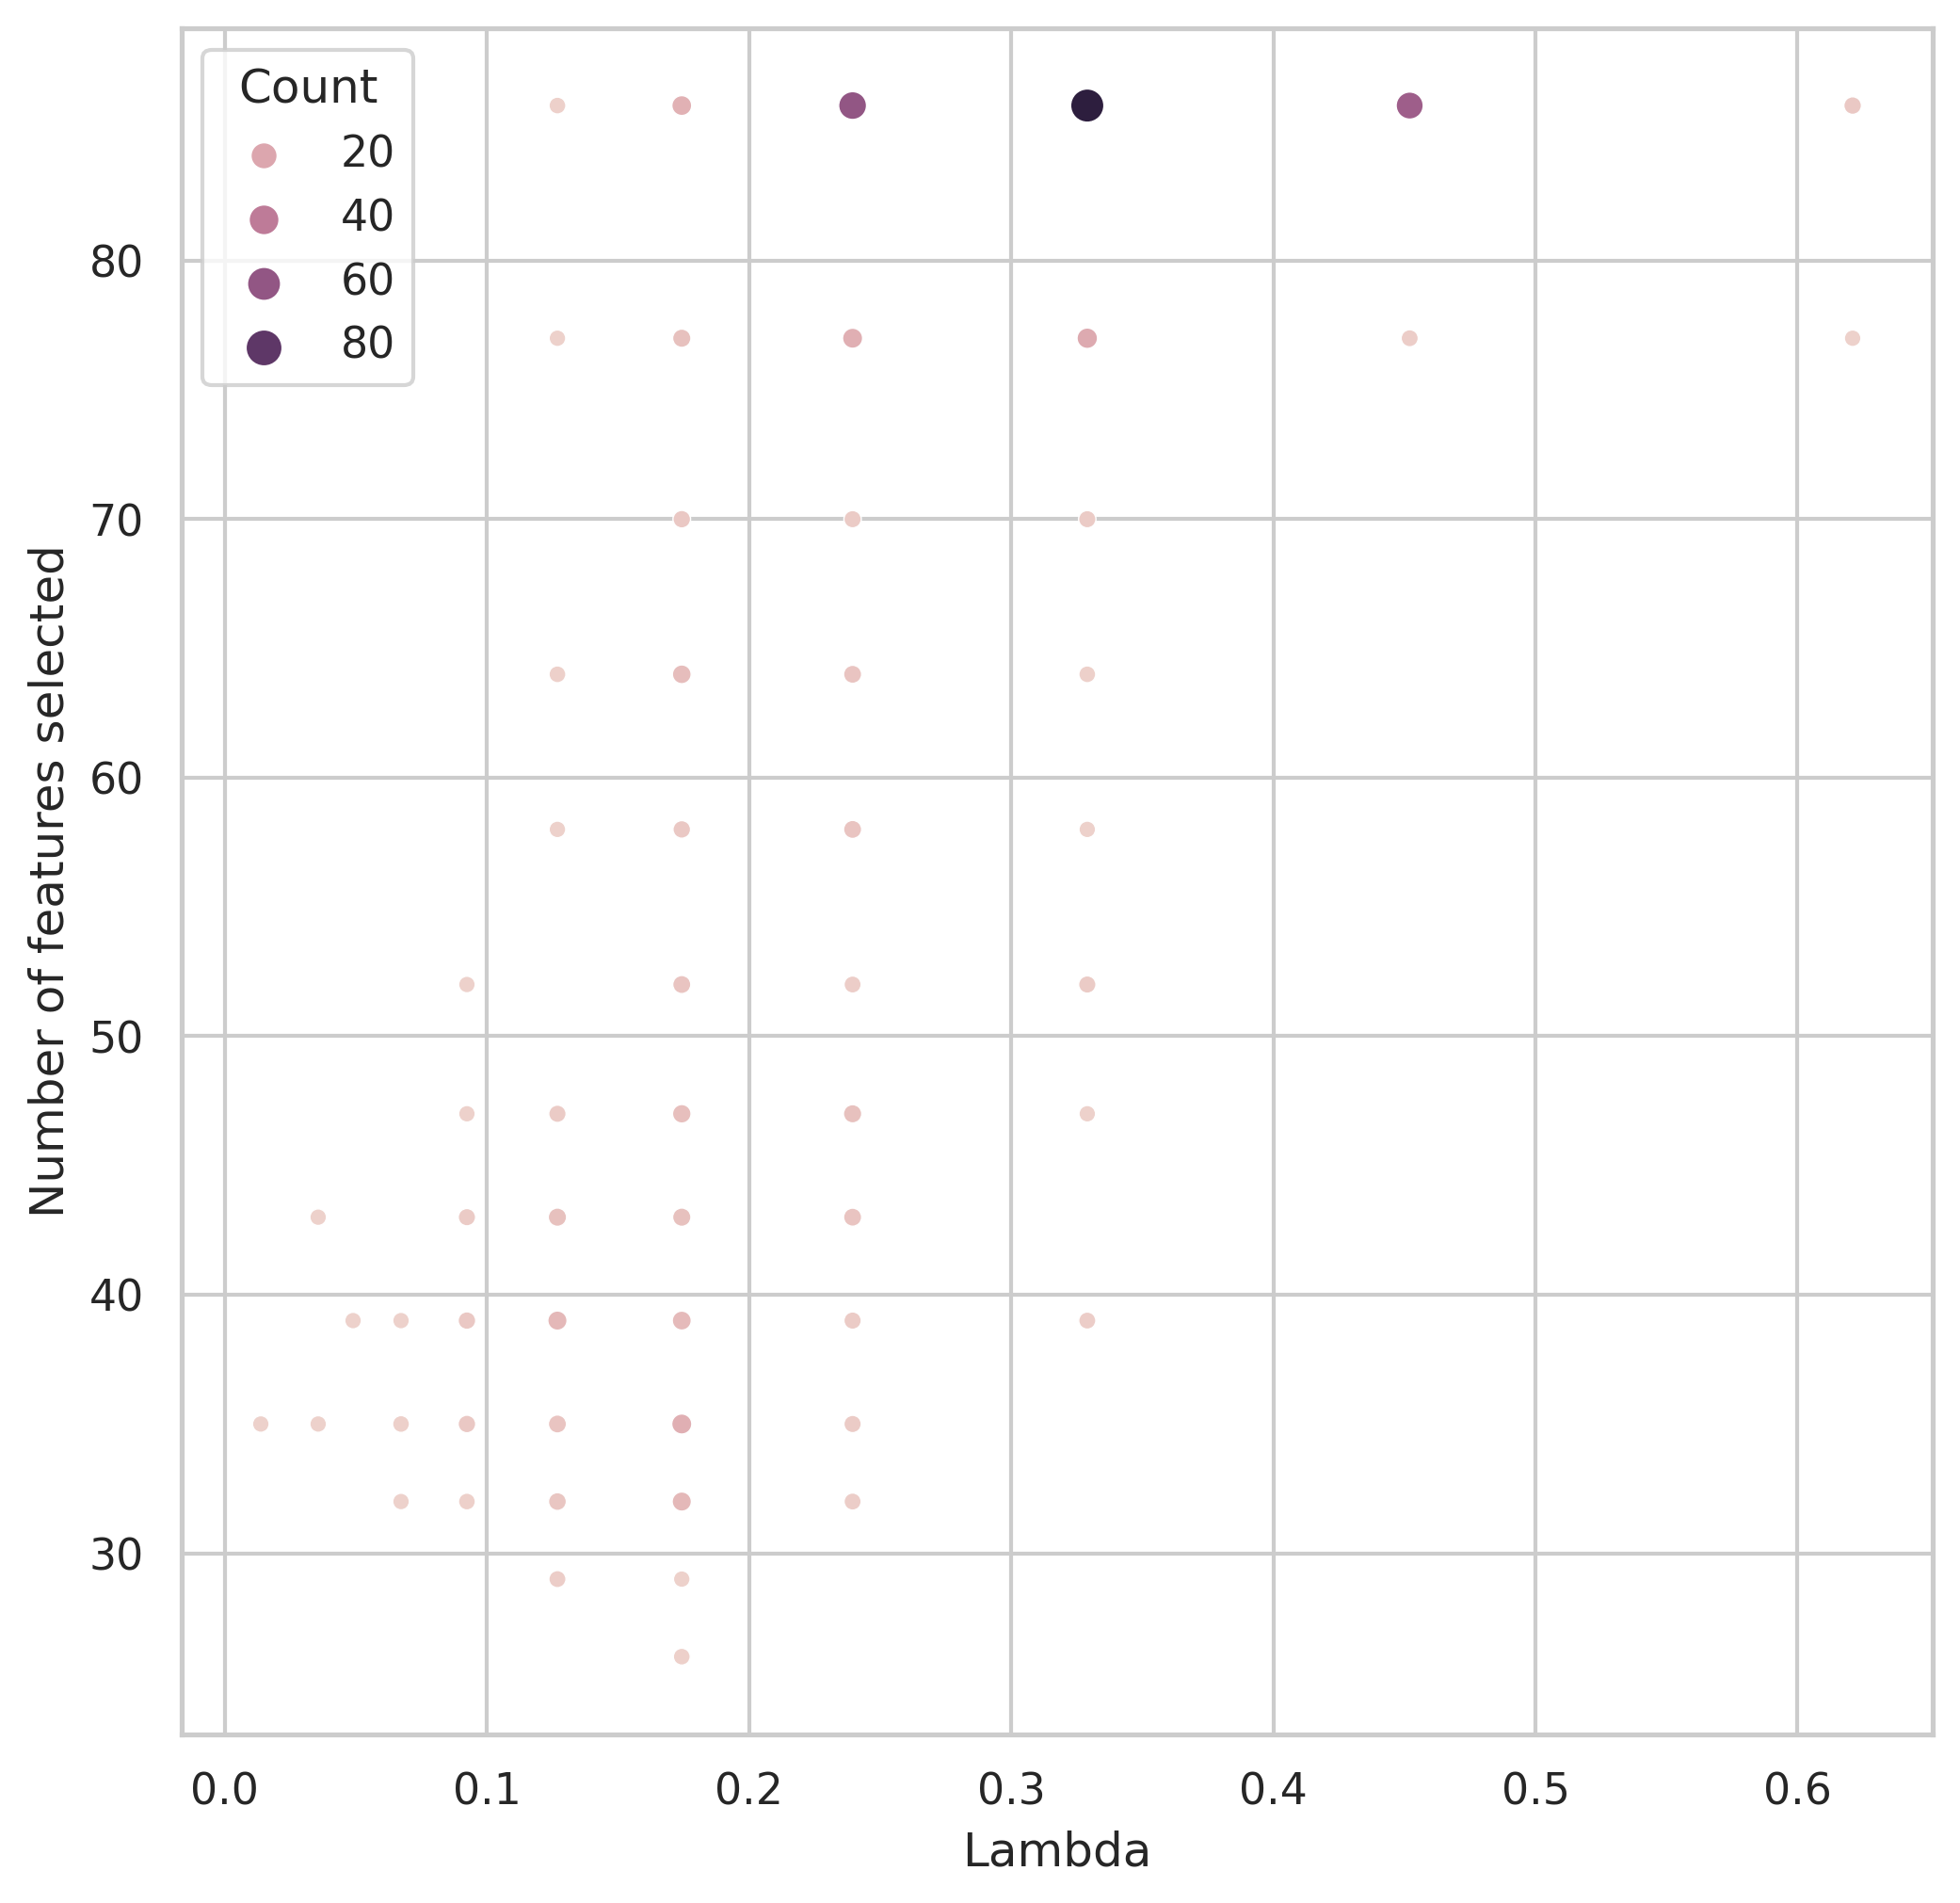
\includegraphics[width=1\linewidth]{figures/fs86subj_normed_motor_scores_chacovol_acutechronic_ridge_crossval1nfeats_lambdas.png}
  \caption{Number of features selected vs. lambda (amount of regularization) for model using ChaCo scores with the FreeSurfer 86-region atlas, acute and chronic subjects together in the training dataset, predicting noromed motor scores. Distribution is showing all outer folds (i.e. 500 outer folds, 5 folds x 100 permutations)}
  \label{fig:sfig1}
\end{subfigure}
\begin{subfigure}{0.5\textwidth}
  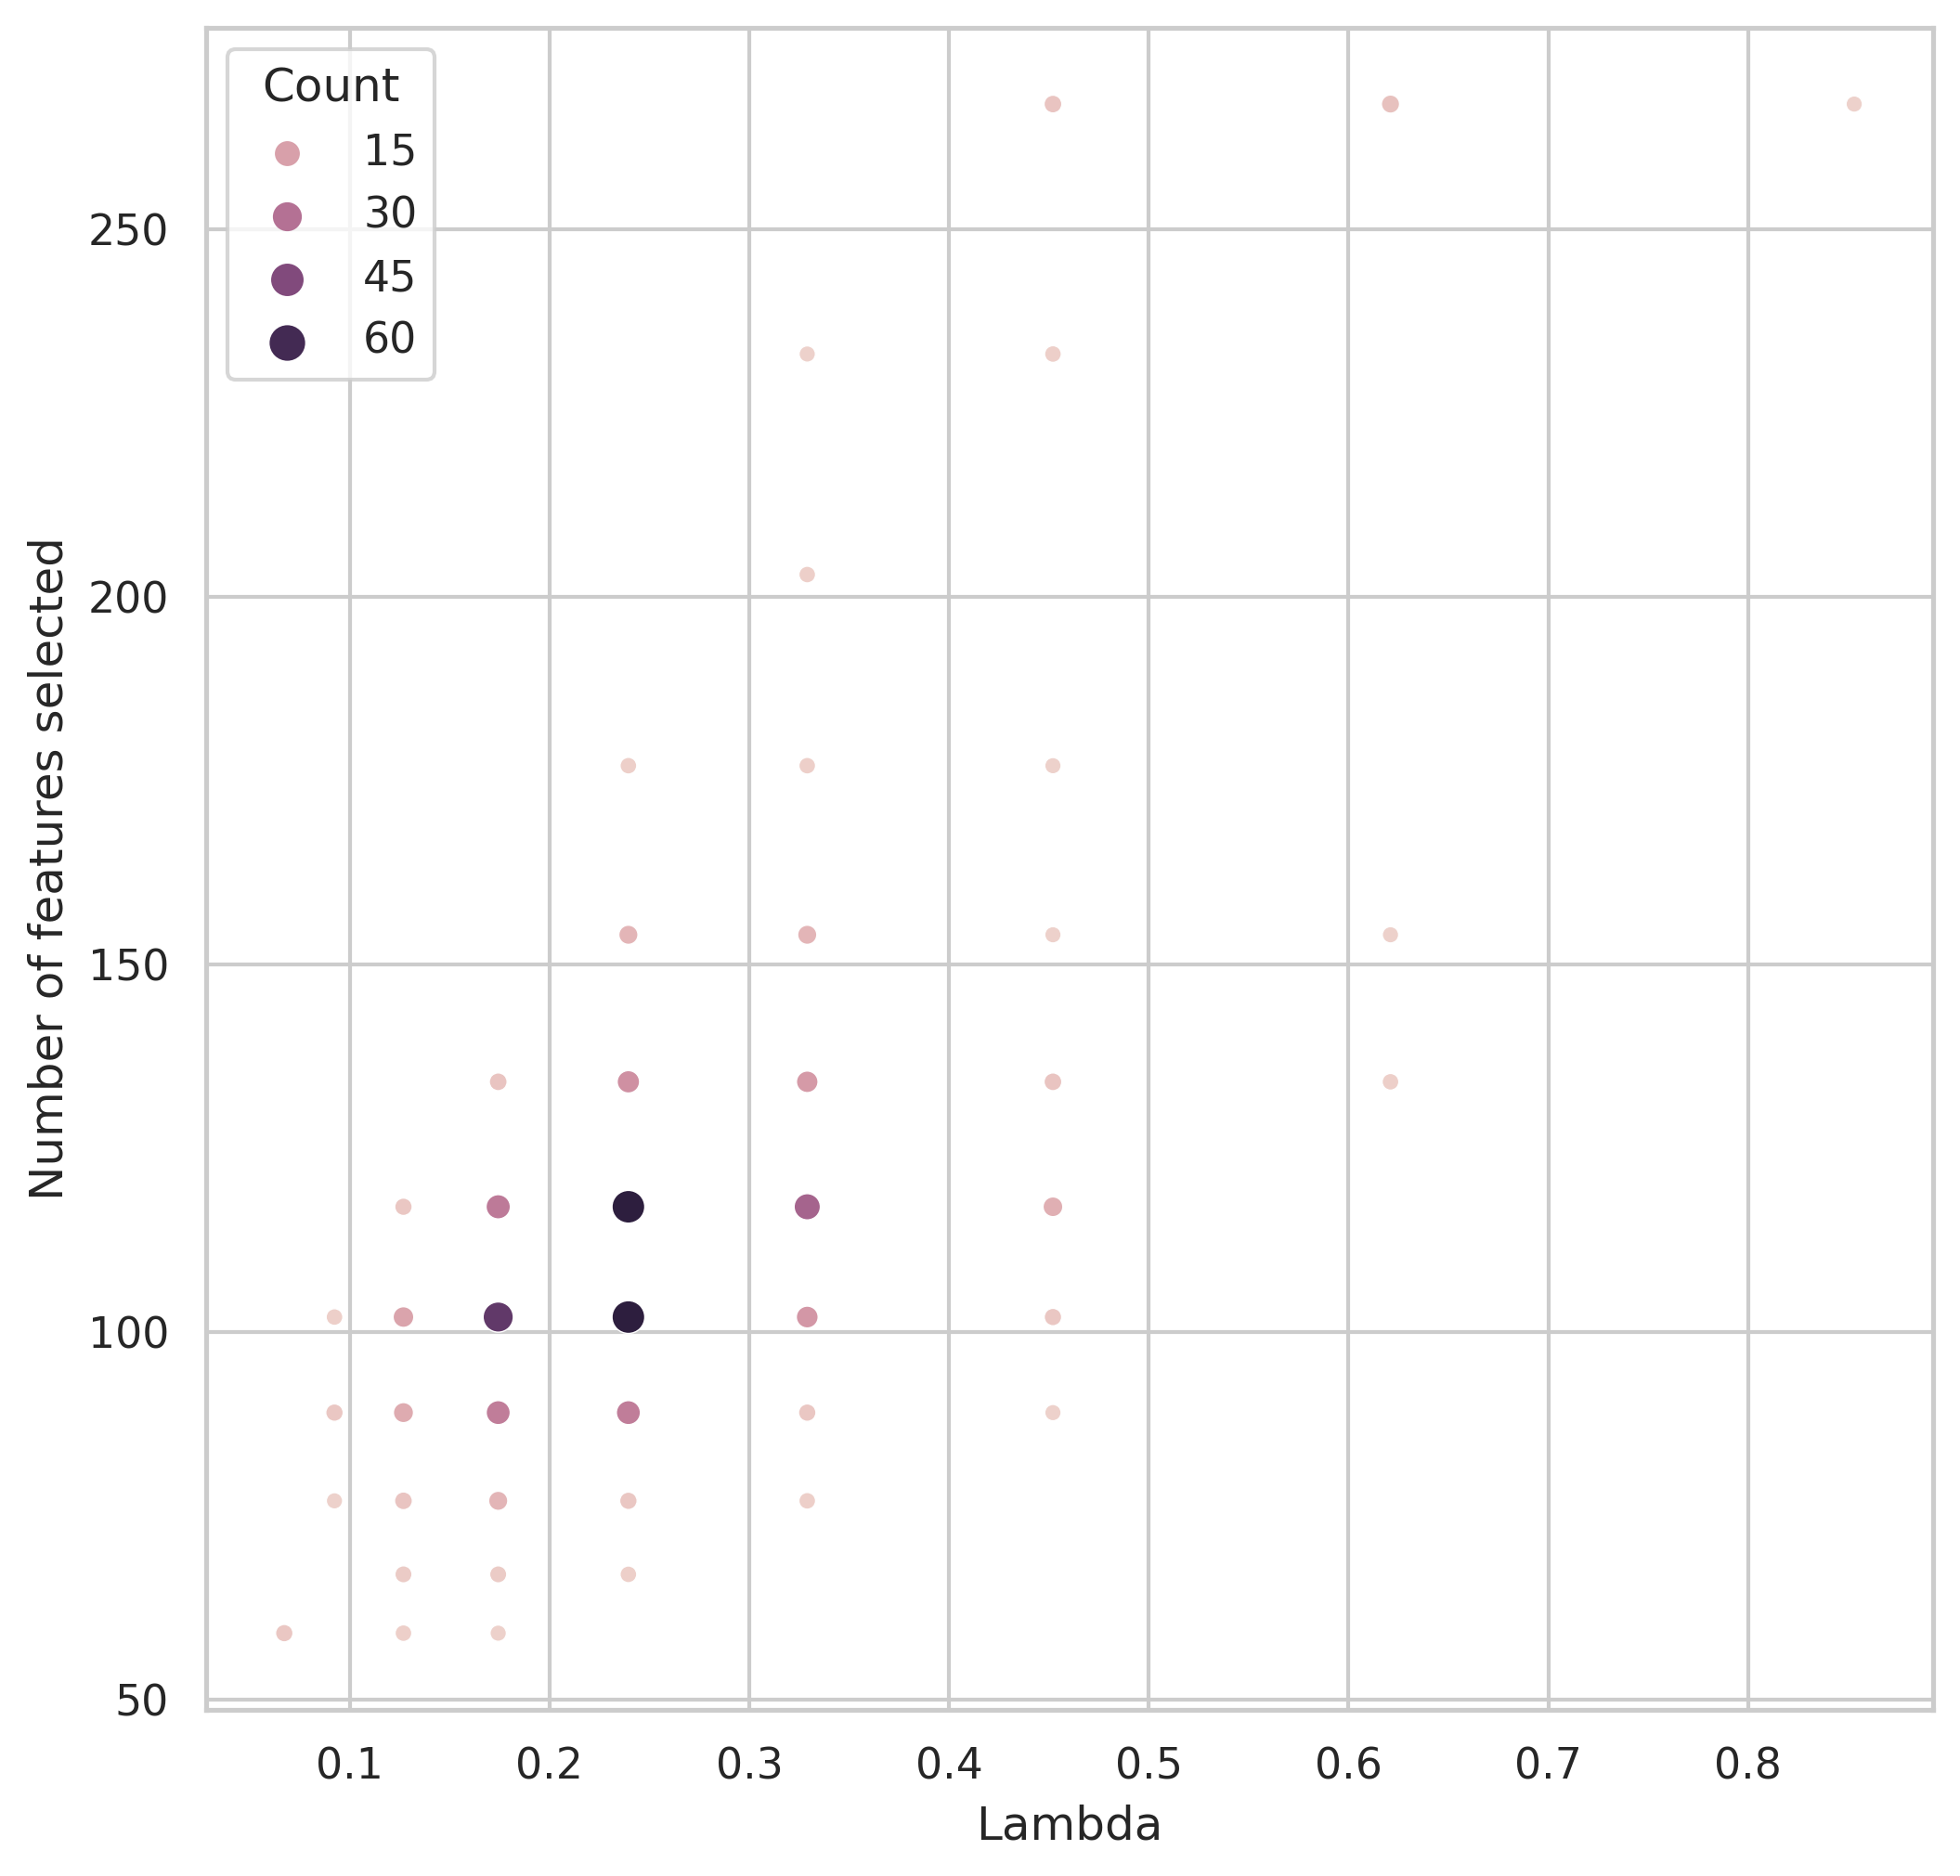
\includegraphics[width=1\linewidth]{figures/shen268_normed_motor_scores_chacovol_acutechronic_ridge_crossval1nfeats_lambdas.png}
  \caption{Number of features selected vs. lambda (amount of regularization) for model using ChaCo scores with the Shen 268-region atlas, acute and chronic subjects together in the training dataset, predicting normed motor scores.Distribution is showing all outer folds (i.e. 500 outer folds, 5 folds x 100 permutations)} 
  \label{fig:sfig2}
\end{subfigure}
\caption{Distribution of number of features selected in ChaCo models (fs86 left, shen268 right) vs. amount of regularization.}
\label{lambda_kappa}
\end{figure}


\begin{figure}[ht]
\centering
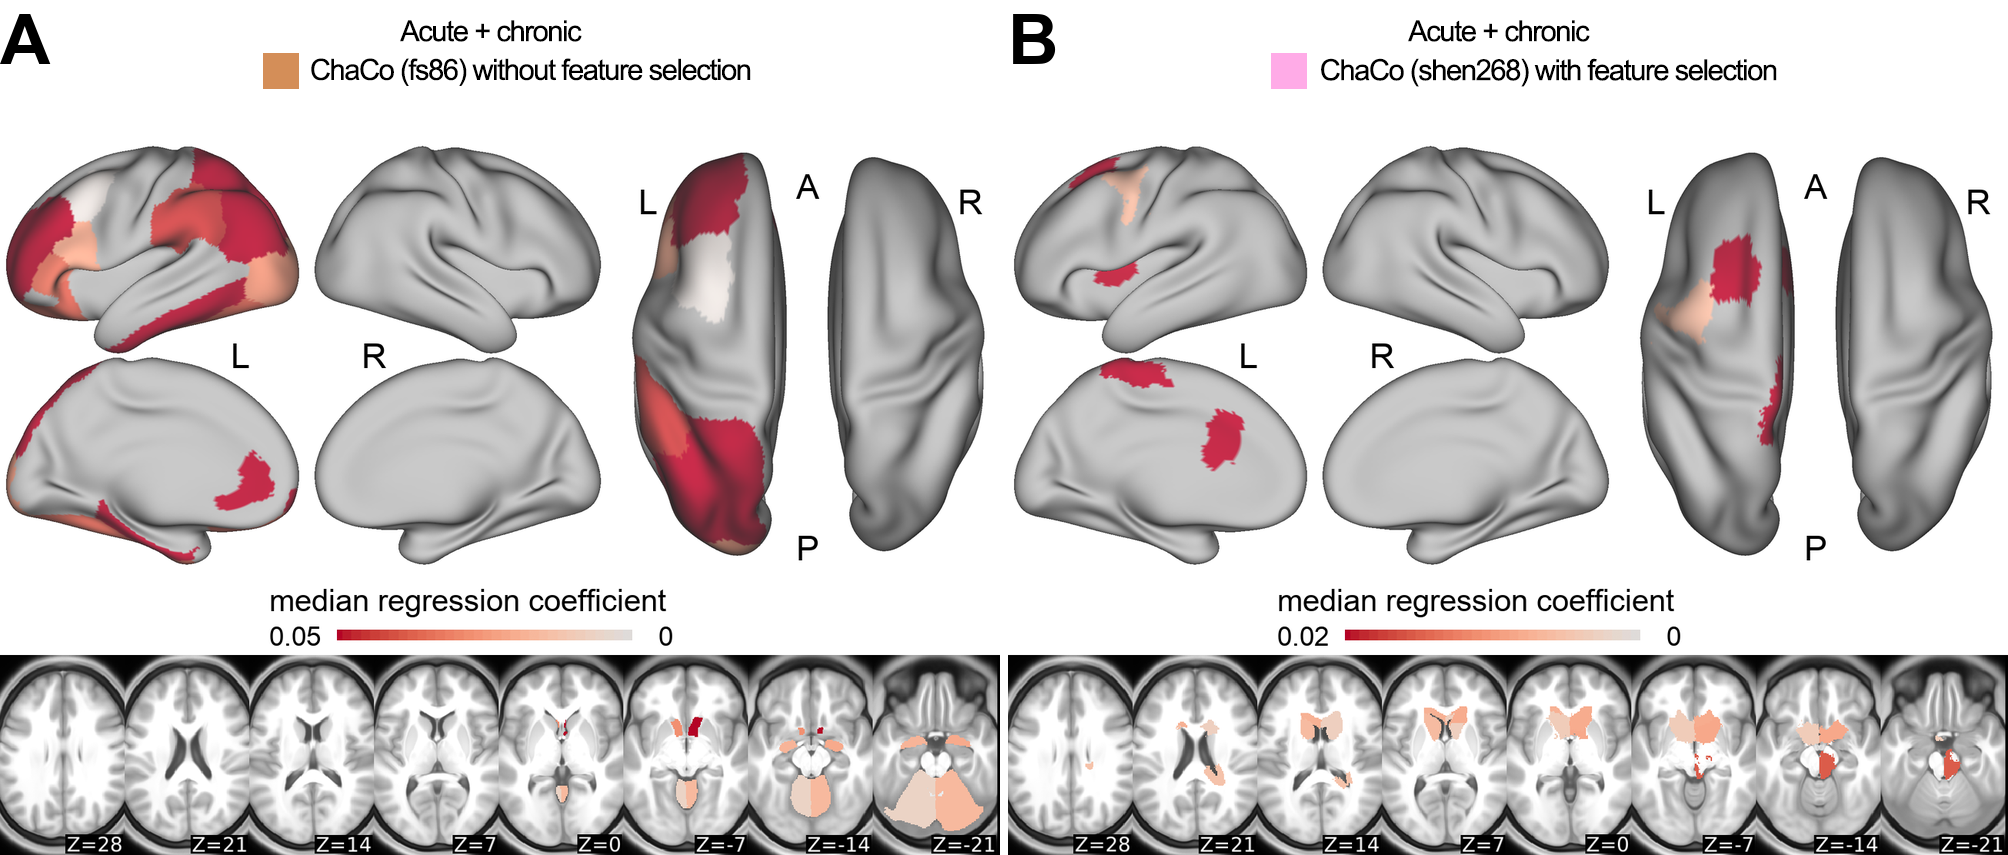
\includegraphics[width=1\linewidth]{figures/Analysis1_posweights.png}
\caption{Positive regression coefficients for the top two best performing models (ChaCo-fs86 without feature selection, shen268 with feature selection).}
\label{analysis1_posweights}
\end{figure}


\end{document}